\documentclass{article}

% if you need to pass options to natbib, use, e.g.:
    \PassOptionsToPackage{numbers, compress}{natbib}
% before loading neurips_2020

% ready for submission
% \usepackage{neurips_2020}

% to compile a preprint version, e.g., for submission to arXiv, add add the
% [preprint] option:
    \usepackage[preprint]{neurips_2020}

% to compile a camera-ready version, add the [final] option, e.g.:
    % \usepackage[final]{neurips_2020}

% to avoid loading the natbib package, add option nonatbib:
    %  \usepackage[nonatbib]{neurips_2020}

\usepackage[utf8]{inputenc} % allow utf-8 input
\usepackage[T1]{fontenc}    % use 8-bit T1 fonts
\usepackage{hyperref}       % hyperlinks
\usepackage{url}            % simple URL typesetting
\usepackage{booktabs}       % professional-quality tables
\usepackage{amsmath}
\usepackage{amsfonts}       % blackboard math symbols
\usepackage{nicefrac}       % compact symbols for 1/2, etc.
\usepackage{microtype}      % microtypography
\usepackage{xcolor}
\usepackage[pdftex]{graphicx}
\usepackage{lineno}
\usepackage{multirow}
\usepackage{hhline}
\usepackage{subfig}
\usepackage{ulem}
\title{Machine Learning Enhancements to Particle Physics Simulations to Reduce Computational Complexity}



% The \author macro works with any number of authors. There are two commands
% used to separate the names and addresses of multiple authors: \And and \AND.
% Using \And between authors leaves it to LaTeX to determine where to break the
% lines. Using \AND forces a line break at that point. So, if LaTeX puts 3 of 4
% authors names on the first line, and the last on the second line, try using
% \AND instead of \And before the third author name.

\author{%
  Robert Johnston \quad Sangbaek Lee \quad Patrick Moran   \\
  Laboratory for Nuclear Science\\
  Massachusetts Institute of Technology\\
  Cambridge, MA 02139 \\
  \texttt{\{robertej, sangbaek, moranp\}@mit.edu} \\
  % examples of more authors
  % \AND
  % Coauthor \\
  % Affiliation \\
  % Address \\
  % \texttt{email} \\
  % \And
  % Coauthor \\
  % Affiliation \\
  % Address \\
  % \texttt{email} \\
  % \And
  % Coauthor \\
  % Affiliation \\
  % Address \\
  % \texttt{email} \\
}

\begin{document}

\maketitle
%\linenumbers

%For initial proposal
%
%%\begin{abstract}
		%Pat's original email
		%In our experiment (CLAS12 at Jefferson Lab), we have event generators that simulate a large number of particle physics events, each of which consist of a number of kinematic variables.
		%The output of these event generators are then passed to another simulation framework that simulates these generated events in the detector geometry of the experiment. 
		%This latter process is very time-consuming given the large number of events that we want to reconstruct in our detectors.
		%We would like to develop a machine learning project that can train on the generated events and reconstructed events, and then predict the output of reconstruction based on the kinematic variables of the generated event.
		%This would allow us to reconstruct only a small amount of generated events through the reconstruction framework, thus drastically reducing the computing time needed for our research.
%% 		An electron-proton scattering experiment has been performed in the CLAS12 detector at the Thomas Jefferson National Accelerator Facility in order to probe the three-dimensional structure of the proton.
%%         Yields of scattered particles into the detector are determined by the types of interactions between incoming electrons and stationary protons.
%%         To understand the underlying physical processes observed in the experiment, the detector acceptance, which is the ratio of the number of events that are detected to the number that are produced, should be precisely estimated. 
%% 		The traditional method is to generate simulated data describing physical processes based on existing knowledge, then to pass these events to the Geant4 software package to simulate their interactions in the detector material.
%% 		A novel method to predict the output of reconstruction based on the kinematic variables of the generated events is described in this project.
%% 		This work is expected to drastically reduce the computing time needed for detector acceptance studies.
%%\end{abstract}


% Evaluation metrics for project proposal (10 points)
% Previous work and references: 2 points
% Understanding the problem, it’s formulation, and goal: 2 points
% Dataset to be used or collected, method or algorithm proposed: 2 points
% Well defined evaluation criteria: 2 points
% Writing clarity and structure: 2 points

% Questions you may answer when writing your proposal:
% What do you want to do? What question are you answering?
% What data will you use? Give a specific description of the data
% and confirm that you already have the data in hand at this point.
% What is your motivation? Formulate your problem as a machine learning problem.
% What methods will you try and compare?
% What computational resources will you use? Think about time and feasibility.
% Relevant related work? (brief summary)
% What is your project plan? You may include key steps and rough internal deadlines for each step.
% What are the risks? What might turn out to be more difficult than you anticipated? And how might you mitigate these risks?
%\linenumbers

%\section{Proposal}
% What do you want to do? What question are you answering?
Large scale particle physics experiments use humankind's largest machines to study nature at the smallest scales. One such experiment, called CLAS12 in Virginia at the Thomas Jefferson National Accelerator Facility (JLab) (\citet{BURKERT2020163419}), collides ultrarelativistic electrons moving only 1 m/s slower than the speed of light into an ultracold bunch of hydrogen to glean information about the substructure of the proton. The electrons interact with protons as described by quantum field theory, which can produce photons that, along with the starting electron and proton, are known as a final state. In particular, two photons, one electron and one proton in the final state is known as Deeply Virtual $\pi^0$ Production (DV$\pi^0$P), and this process is currently under detailed study as its properties are related to the mechanical properties of the proton (\citet{PhysRevD.55.7114}). 

%This is a continuation of the above paragraph, getting to answering "what is it you want to do" - I think what we need to answer is - we want to repalce GEANT4 with a generative model" 
The purpose of the CLAS12 detector is to detect the individual particles of this and other final states by recording the electrical signals produced when they pass through specific materials, which are then stored digitally and analyzed with reconstruction algorithms. In practice, there are many difficulties in reliably detecting and reconstructing particle paths, so computational methods have been developed to better understand detector and analysis algorithm's responses. Typically, real data is compared with the output of detailed simulations of the experiment, wherein Monte-Carlo (MC) methods are used to walk simulated particles through a detector system in many small time steps (\citet{PhysRevLett.115.212003, 10.1093/ptep/ptaa104}). However, this simulation method is very computationally expensive, especially for our particular physics experiment and process. Our goal is to use a generative machine learning model to mimic the output of the MC simulation and reconstructions, thus reducing computation time.


% What data will you use? Give a specific description of the data
% and confirm that you already have the data in hand at this point.
The standard simulation consists of two steps. First, we generate a data set of particle features - momenta and other properties - based on a combination of field-theoretic functions and empirical physics models, which creates an 'event' of a realistic four-particle final state from the DV$\pi^0$P process. This generation is very simple once the physics process has been defined, and well known and studied generators already exist\footnote{https://github.com/JeffersonLab/clas12-mcgen/}, and are very computationally inexpensive - 1 million events can be produced in less than a minute. The second step is for each event, walk all four particles through the simulated detector setup using the GEANT4 package (\citet{AGOSTINELLI2003250}). The output from this step is our four particles that we began with, but with their features smeared out. This second step is the one we are trying to supplement, as it would take about 5,000 hours on a single core machine to process 1 million events. However, through HPCC we have produced so far 100 M generated (step 1) and simulated (step 2) events that can be used for algorithmic training. 


% What is your motivation? Formulate your problem as a machine learning problem.
To describe the data structure, we start from a toy model, a baseball game with one pitcher and one catcher. In one ``inning", the pitcher throws a ball four times in a row, knowing the ball's speed and direction in spherical coordinates (speed, polar angle $\theta$, azimuthal angle $\phi$) in the beginning. The catcher also records the four ball's speed and directions in $x^{i}$'s in 4$\times$3 matrices. In $i$-th inning, the pitcher and the catcher have the data $z^{i}$ and $x^i$ as 4$\times$3 matrices. The catcher may catch all of the balls correctly like $x^0$, and sometimes miss some balls like $x^1$ (Fig.~\ref{data}-a). One wants to collect the pair of $z^i$ and $x^i$, but notices that hiring a catcher is far more expensive than hiring a pitcher.

\begin{figure}[!ht]
 \centering
   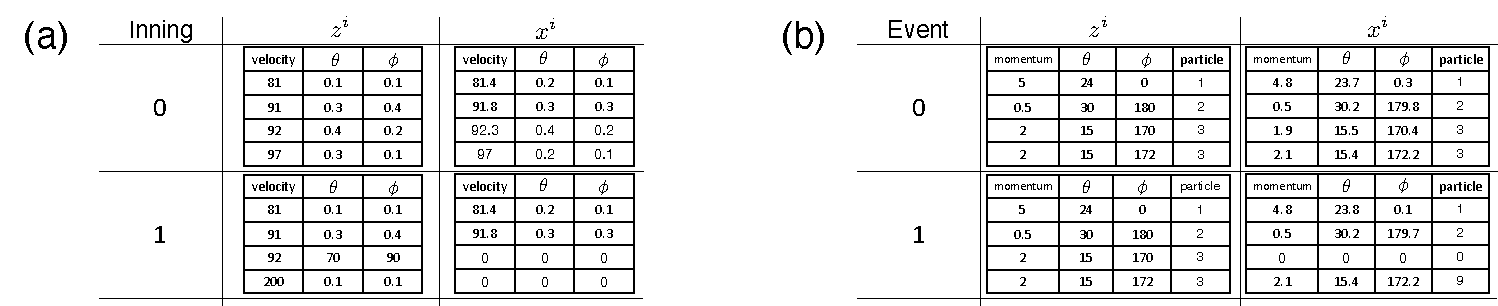
\includegraphics[width=0.8\linewidth]{dataDescription.pdf}
  \caption{The first two rows of (a) toy model data with a pitcher and a catcher, (b) actual data with particles.}
  \label{data}
\end{figure}

In our data, the pitcher's record corresponds to our generated event particle features, and the catcher's record corresponds to the results of MC simulation. The results of each simulation are essentially encoded particle kinematics. One particle has a 4 dimensional vector, where 3 dimensions come from (momentum, polar angle $\theta$, azimuthal angle $\phi$) and another one from particle species. The example of the first two events are in Fig.~\ref{data}-b. In summary, $x^i$'s are in $n\times\{4\times$4\}, and $z^i$'s are also in $n\times\{4\times$4\} dimension, when $n$ is total number of events. Since determining $x^i$ by calculating incremental timesteps is very computationally expensive as mentioned earlier, we aim to replace this step with a generative model that takes input as $z^i$, and outputs $x^i$.

% Relevant related work? (brief summary)
There have been some attempts to generate $x^i$'s using several generative models including the GAN (\citet{Paganini2017}) for different particle experiments. However, the GAN is not an optimal choice for this problem as our goal is to generate a large output dataset and only require relatively low fidelity for each individual output $x^i$, rather than generate only a handful of very high fidelity output events. More recently, the normalizing flow (NF) (\citet{papamakarios2019normalizing}) was studied as a generative model suitable for producing a large number of items that pertain to a very particular distribution of $g: z\rightarrow x$ (\citet{9089305}). \citet{PhysRevD.101.076002} showed that the Nonlinear Independent Component Estimation (NICE) (\citet{Dinh15}) as NF performed well by comparing the technique to existing methods in terms of efficiencies that was defined as average weight during the generation.

% What methods will you try and compare?
We will use a NF model which takes $Z=\{z^i\}$ with the base distribution $p(z)$, and $X=\{x^i\}$ with the target distribution $p(x)$. The mapping in the generative direction is defined as $g:Z\rightarrow X$ with its inverse in normalizing direction $f:X\rightarrow Z$. The distributions have following relation with $f$ and $g$: $p(x)= p(z)|\frac{\partial f}{\partial x}| =  p(z)|\frac{\partial g}{\partial z}|^{-1}$. Technically, it is useful to define $g$ and $f$ as composite bijective functions, $g= g_N \circ g_{N-1}\circ ... \circ g_1$, and $f= f_1 \circ ... \circ f_{N-1} \circ f_N$. With this, it is possible to perform the exact log-likelihood evaluation: $\log p(x) = \log p(z) + \sum\limits_{i=1}^N \log|\frac{\partial f_i}{\partial z_i}|$ where $z_i$ is the $i$-th intermediate flow as $z_i=g_i \circ ... \circ g_1(z) = f_{i+1}\circ ...f_N(x)$. Among possible flow models, we plan to use NICE, and will compare the NF-generated data to the output of the MC simulation.

% What computational resources will you use? Think about time and feasibility.
Regarding the computational feasibility of this project, our group has access to several powerful computing farms, such as LHC Tier-2 \footnote{monitored at http://www.cmsaf.mit.edu/condor4web/}, JLab iFarm \footnote{monitored at https://scicomp.jlab.org/scicomp/index.html\#/farmJobs/activeJob}, and EAPS - MGHPCC \footnote{https://www.mghpcc.org/}. Data storage is not a limiting factor, as 1 GB alone stores 10M $z^i$ - $x^i$ pairs. We propose the following project timeline:\\
\textbf{March 31} Match components of the NICE to our data at pseudo code level, begin implementation \\
\textbf{April 10} - Have basic working example, begin improving and optimizing project \\ 
\textbf{April 25} Conclude developing project flow, begin generating and validating final data \\
\textbf{May 4} - Conclude production run of project, begin finalizing reports.
%OLD:
%We, as members of the MIT Hadronic Physics group, are granted access to MIT clusters such as an HTCondor farm, LHC Tier-2 \footnote{monitored at \url{http://www.cmsaf.mit.edu/condor4web/}}, and a slurm farm, EAPS cluster. Some farms external to MIT can be accessed using OSG for CLAS12 collaboration. The ifarm also offers some computing power \footnote{monitored at \url{https://scicomp.jlab.org/scicomp/index.html\#/farmJobs/activeJob}}. These farms are operating anytime. Especially, the EAPS cluster runs without any delay, and supports disk space of 2 TB quota. For $n$ = 5M, $Z$ and $X$ take roughly 400 MB space.

% What is your project plan? You may include key steps and rough internal deadlines for each step.
%\begin{center}
%\begin{tabular}{ c c c }
%\textbf{Date} & \textbf{Project Milestone} \\ 
%  \textbf{March 31} & Match all components of the NICE to our data in pseudocode level \\
%  \textbf{April 10} & Write an actual code, and have minimal working example on small dataset  \\  
%  \textbf{April 25} & Have working example on full scope of problem \\ 
%  \textbf{May 4} & Conclude production run of project, begin finalizing reports
%\end{tabular}
%\end{center}

% What are the risks? What might turn out to be more difficult than you anticipated? And how might you mitigate these risks?
One anticipated difficulty in this project is that any NF model requires $g$ to be invertible and differentiable. This is fulfilled if we take $x^i$ only when fully reconstructed, like event 0 of Fig.~\ref{data}-b. If not all, but some particles are missing, like event 1 of Fig.~\ref{data}-b, and we encode the momentum feature to 0, differentiability is not guaranteed. Moreover, if all particles are missing, we surely lose invertibility. To address this, we will being work only with fully reconstructed events, which make up the great majority of our interest.  For the events with missing particles, we can encode their momenta to (0, 0, 0) +  small random noises, which can be finally decoded as missing particles, but it is not clear at this stage if this will be a successful approach. If it is not, we will still be able to learn a great deal about our detector by examining the fully reconstructed cases.
%\quad The overarching goal of this project is to provide a correction factor for detector acceptance in our experiment. This will be a large, overall normalization factor, and as our thesis goal is to measure absolute quantities (rather than ratios) this project runs the risk of providing an inaccurate acceptance correction term, which would then yield a significantly shifted final result. This can be mitigated by extensive cross-validation of results, and can be extensively verified by running large simulations in a small region of phase space to create new data for comparison purposes.

%\quad On a more technical level, as this is a very high dimensional problem, it could be difficult to engineer an efficient algorithm for this process. This issue could be mitigated by building up to our actual process in incremental steps, e.g., trying to build an algorithm that will be able to efficiently predict the outcome of just one simulated particle, and then build onto more complex initial and final states. If we are not able to realize our full initial and final state mappings to yield correction factors, we would still be able to gain useful insight by understanding better how single particles, e.g. electrons, traverse through our detector. 



%garbages previously submitted <3
%Since the experimental discovery of the proton by Ernest Rutherford over 100 years ago, there have been various attempts to reveal its internal structure. Yet, its three dimensional profile is still elusive. Measurements on deeply virtual exclusive processes (DVEP) from electron-proton scattering are one proposed way to project the proton structure [\citet{PhysRevD.55.7114}]. In the CLAS12 detector at Thomas Jefferson National Accelerator Facility (JLab), experimental data has been taken of these and other processes [\citet{BURKERT2020163419}].

%Ideally, an event should consist of initial and final states. This is not always true because particles in final states are stochastically detected, depending on their kinematics and detector efficiencies.

 %In this work, we match events $x^i$'s into binary labels $y^i$'s: (\textit{A}) events where every particle gets detected and is correctly classified as the final state of the exclusive process of interest; (\textit{B}) events that fail to be classified as the final state but come from the exclusive process. The goal of this work is to estimate the detector acceptance, the number of \textit{B} events based on measurements of \textit{A} events.  %; and (\textit{C}) events that are not related to the exclusive processes. 
 
 %commented by Sangbaek
 %In the real experiment, the number of events labelled as \textit{A} can be measured. On the other hand, it is hard to estimate the number of events labelled as \textit{B} from the experiment. One widely accepted way is to use a Monte-Carlo simulated data set to estimate the detector acceptance [\citet{PhysRevLett.115.212003, 10.1093/ptep/ptaa104}]. The simulation consists of two steps. The first step is to generate physical events by the Metropolis-Hastings algorithm. The second step is to pass these events to the GEANT4 package [\citet{AGOSTINELLI2003250}], which simulates the interaction between the final states and detectors. The experimental data is stored in the JLab computing facility, which can be accessed by ssh-ing into their farm, named ifarm. Simulated data can also be achieved using computing facilities connected to Open Science Grid (OSG), including MIT farms. The simulated data of a few million events are already achieved, more amounts of simulated data can be easily taken from OSG. For example, in one day, we can roughly simulate 100M events of data.


%Unlike our physics process of interest, which has a high dimensional phase space, most physics final states are considerably more simple, and as such, it has been easier for previous experiments to just run GEANT4 simulations, rather than use machine learning to determine acceptance corrections. As such, work exactly similar to our proposed project has not yet been performed, but machine learning techniques are ubiquitous throughout our research community. Convolutional neural networks (CNN) have been explored by the ALICE collaboration at CERN to supplement particle identification algorithms [\citet{Viljoen2020}], essentially analogous to our project except we will classify whole events, rather than individual particles. Moreover, research is ongoing with replacing traditional GEANT4 simulations with ML boosting to produce 'fast simulations' wherein computationally expensive simulation over dense detector materials are replaced with GANs and VAEs to yield orders of magnitude speedup in simulation time [\citet{Albertsson2018}, \citet{Paganini2017}].


%There are difficulties in estimating the detector acceptance using simulated data. Generally, this type of computing takes too much time to collect significant statistics. Also, sometimes kinematics of label \textit{A} events in simulation may not match with label \textit{A} events in the real experiment. Also, the ratio from simulated data largely depends on theoretical model for probability distribution that was used for Metropolis-Hastings algorithm. Finally, the acceptance only depends on particle kinematics, so it is not efficient to run each process for large statistics. Now this task can be re-defined as a machine learning problem in following way. We have particle momenta in the experimental and simulated data. As indicated earlier, the detector acceptance, despite being stochastic, must be a function of momenta of final states. We take momenta of final states as feature vectors. Each event has label of detector acceptance $\in$ [0, 1], by definition. We define training data sets as simulated data, and a test data set as experimental data. We keep cross validate with several training data sets, and apply our algorithm to the test data.

%Like previous works, we propose using CNN and GAN for this project. First, we will try regression with CNN with simulated data, and test on experimental data. Second, we will try GAN to mimic our simulated data to get more statistics without performing more simulation. We will estimate the detector acceptance with GAN data, and compare the detector acceptance for the experimental data.


%For Milestone Meeting
%
\iffalse
CHECKLIST:
 - 3 pages + references
 - (DONE) Title
 - Abstract
 - Introduction - 7 pts
  -- Introduction (2 points)
  -- Related work and references (2 points)
  -- Problem Formulation, technical depths, innovation (3 points)
 - Methods - 5 pts
  -- Methods, technical depth and innovation, architecture and design (5 points)
 - Results - 8 pts
  -- Preliminary results, Github repo, data, code correctness, readability (8 points)
 
 - Submit to Canvas by 4.12 at 9 AM
 - Resubmit Milestone after meeting by (Friday 4.16?) at 9 AM
\fi

\begin{abstract}
We demonstrate a proof of principle for using a normalizing flow to learn a physics process's probability distribution to effectively sample more data. The training data set has 5 million data points of 12 features for both $z$ and $x$ where the normalizing flow transforms $z$ to $x$. In this work, we take as input a constant 2D logistic distribution instead of $p(z)$, and examine whether the flow model can learn the transformation to $p(x)$. For simplicity, at this stage we demonstrate the method using only two features of $x$, and observed a reasonable agreement between the given physics sample and the newly-sampled data using the flow model.
\end{abstract}
\section{Introduction including Related Works }
%(we can now cite Stan's work! \textcolor{red}{did he already submit his thesis to DSpace MIT?})

Large scale particle physics experiments use humankind's largest machines to study nature at the smallest scales. One such experiment, called CLAS12 in Virginia at the Thomas Jefferson National Accelerator Facility (JLab) (\citet{BURKERT2020163419}), collides ultrarelativistic electrons moving only 1 m/s slower than the speed of light into an ultracold bunch of hydrogen to glean information about the substructure of the proton. In particular, two photons, one electron and one proton in the final state is known as Deeply Virtual $\pi^0$ Production (DV$\pi^0$P), and this process is currently under detailed study as its properties are related to the mechanical properties of the proton (\citet{PhysRevD.55.7114}).

Typically, real data is compared with the output of detailed simulations of the experiment, wherein Monte-Carlo (MC) methods are used to walk simulated particles through a detector system in many small time steps (\citet{PhysRevLett.115.212003, 10.1093/ptep/ptaa104}). The standard simulation consists of two steps. First, we generate a data set of particle features - momenta and other properties - based on a combination of field-theoretic functions and empirical physics models, which creates an `event' of a realistic four-particle final state from the DV$\pi^0$P process. This generation is very simple and computationally inexpensive. The second step is, for each event, walk all four particles through the simulated detector setup using the GEANT4 package (\citet{AGOSTINELLI2003250}). The output from this step is our four particles that we began with, but with their features smeared out. This second step is the one we are trying to supplement, as it would take about 5,000 hours on a single core machine to process 1 million events. However, through HPCC we have produced so far 100 M generated (step 1) and simulated (step 2) events that can be used for algorithmic training. 

The normalizing flow is an effective model to learn a probability distribution $p(x)$ when a sample data set $X=\{x\}$ following the distribution is given. The basic idea is a series of transformation $g_i$'s, which are referred to as flows, transforms a prior probability $p(z)$ distributions into the target distribution $p(x)$. That is
\begin{align}
    \mathbf{x} =& g_N \circ g_{N-1}\circ ... \circ g_1 (\mathbf{z}) \\
    \mathbf{z} =& f_1 \circ ... \circ f_{N-1} \circ f_N (\mathbf{x}) \label{eqn:invertible}
\end{align}
, where $f_{N-i+1}\equiv g_i^{-1}$ following \citet{9089305}'s convention. Both $\mathbf{x}$ and $\mathbf{z}$ are vectors of the same dimension $d$. From the eq.~\ref{eqn:invertible}, $g_i$ requires an invertibility condition. An intermediate flow $\mathbf{z_i}$ is defined as follows.
\begin{align}
\mathbf{z_i} =&g_i \circ ... \circ g_1(\mathbf{z}) \label{eqn:forward}\\
    =&f_{i+1}\circ ...f_N(\mathbf{x}) \label{eqn:backward}
\end{align}
, where the flow is expressed in forward direction at eq.~\ref{eqn:forward}, and in backward direction at eq.~\ref{eqn:backward}. Therefore, $\mathbf{z_{i+1}}=g_i (\mathbf{z_i})$ and $\mathbf{z_i} = f_{N-i+1}(\mathbf{z_{i+1}})$ for one flow, or layer. If the $f_i$'s are differentiable, the PDF evolves as follows.
\begin{align}
 p(\mathbf{z_{i+1}})=& p(\mathbf{z_i})|\frac{\partial f_{N-i+1}}{\partial \mathbf{z_i}}| =p(\mathbf{z_i})|\frac{\partial g_{i}^{-1}}{\partial \mathbf{z_i}}|\\
 \log p(\mathbf{z_{i+1}}) =& \log p(\mathbf{z_i}) + \log|\frac{\partial g_i^{-1}}{\partial \mathbf{z_i}}| \label{eqn:logprob}\\
 \log p(\mathbf{x}) =& \log p(\mathbf{z}) + \sum\limits_{i=1}^N \log|\frac{\partial g_i^{-1}}{\partial \mathbf{z_i}}|.
\end{align}
Eq.~\ref{eqn:logprob} is useful to define the forward and the backward propagation of each layer.
Once the NF model is trained to learn the distribution $g: p(z)\rightarrow p(x)$, it is possible to sample $x$ using sampled $z$. \citet{PhysRevD.101.076002} showed that the Nonlinear Independent Component Estimation (NICE) (\citet{Dinh15}) implementation of NF performs well by comparing the technique to existing methods in terms of efficiencies that are defined as average weight during the generation.

Motivated by \citet{stan}'s work, we use Masked Autoregressive Flows (MAF, \citet{papamakarios2018masked}), which is one of the generalized versions of NICE. The MAF starts from a simple fact that $p(z_{i}) = \prod\limits_{j}p(z_{i,j}|\mathbf{z}_{i,1:j-1})$. The component $z_{i,j}$ is the $j$-th component of $z_i$, and the vector $\mathbf{z}_{i,1:j-1}$ is defined as $\{z_{i, 1}, ..., z_{i, j-1}\}$. The transformation is finally defined as
\begin{align}
    z_{i+1, j}=& \sigma_{i, j} z_{i, j} + \mu_{i+1, j}.
\end{align}
The moments $\mu_{i+1, j}$ and $\sigma_{i, j}$ are the mean and standard deviation of $p(z_{i+1,j}|\mathbf{z}_{i+1,1:j-1})$ ($\equiv p(z_{i+1,1})$ for $j=1$). We train the flows to learn $\mu_{i+1, j}$'s and $\sigma_{i, j}$'s, and sample $p(\mathbf{x})$.

\citet{papamakarios2018masked} presents a good github repository of how to train a NF for a 2-dimensional image. The libraries are very straightforward and use PyTorch. The architecture consists of the two layers of MAF and the 2d normal prior distribution.

\section{Methods}
%We should include our work of generating the data (GEMC) and processing the data (convert to root, pandas, pickle) as these are all non-trivial steps and a good "data pipeline"
The data of 5M `events`, or sets of data points, in this problem has been achieved from Open Science Grid (OSG). The original data format is in ROOT \cite{root}, which is a widely-used format in high energy physics written in C++. There have been improvements in python libraries like uproot \cite{uproot} that can interpret the ROOT data format. The data file has been read using uproot, and saved in pickle, a standard Python library for serializing data \footnote{\url{https://github.com/6862-2021SP-team3/hipo2pickle}}. The pickled data has 5M row, each of which contains the features of four individual particles. Each individual particle has 3 features (magnitude of momentum, polar angle, azimuthal angle), so our sample $x$ has dimensions of $5\text{M}\times12$. The sampled $z$ has the same dimensions, but as sampled data points, not in the analytic distributions. \citet{Dinh15} mentions that the ``prior distribution does not need to be constant and could also be learned." We expect to learn the distribution of sample $z$'s with another NF, and use that distribution of prior in the final results. But we ignore the actual $z$ distributions, and try with the constant distributions at this stage.

\textcolor{red}{change these accordingly} We forked the repository in the organization \footnote{\url{https://github.com/6862-2021SP-team3/pytorch-normalizing-flows}}, and tested the libraries for our purpose. For the proof of the concept, we only use two columns of our data set $x$---the magnitude of electron momentum and the polar angle. We observed a good results when we used logistic distributions as prior, 12 additive alternating coupling layers, 1 output scaling layer.

\section{Preliminary Results}
The distribution in the top left subplot of Figure \ref{fig:a} shows the 2d distribution of the training data. The MAF flow was trained using a 2-dimensional logistic distribution prior, with 5,000 iterations using a sample of 1,000 training data points for each iteration. The meta-parameters of learning rate and weight decay were empirically set to 5$\times$ 10$^{-4}$ and 1$\times$10$^{-9}$, respectively. 

\begin{figure}[!ht]
    \centering
    \begin{minipage}{.5\textwidth}
        \centering
        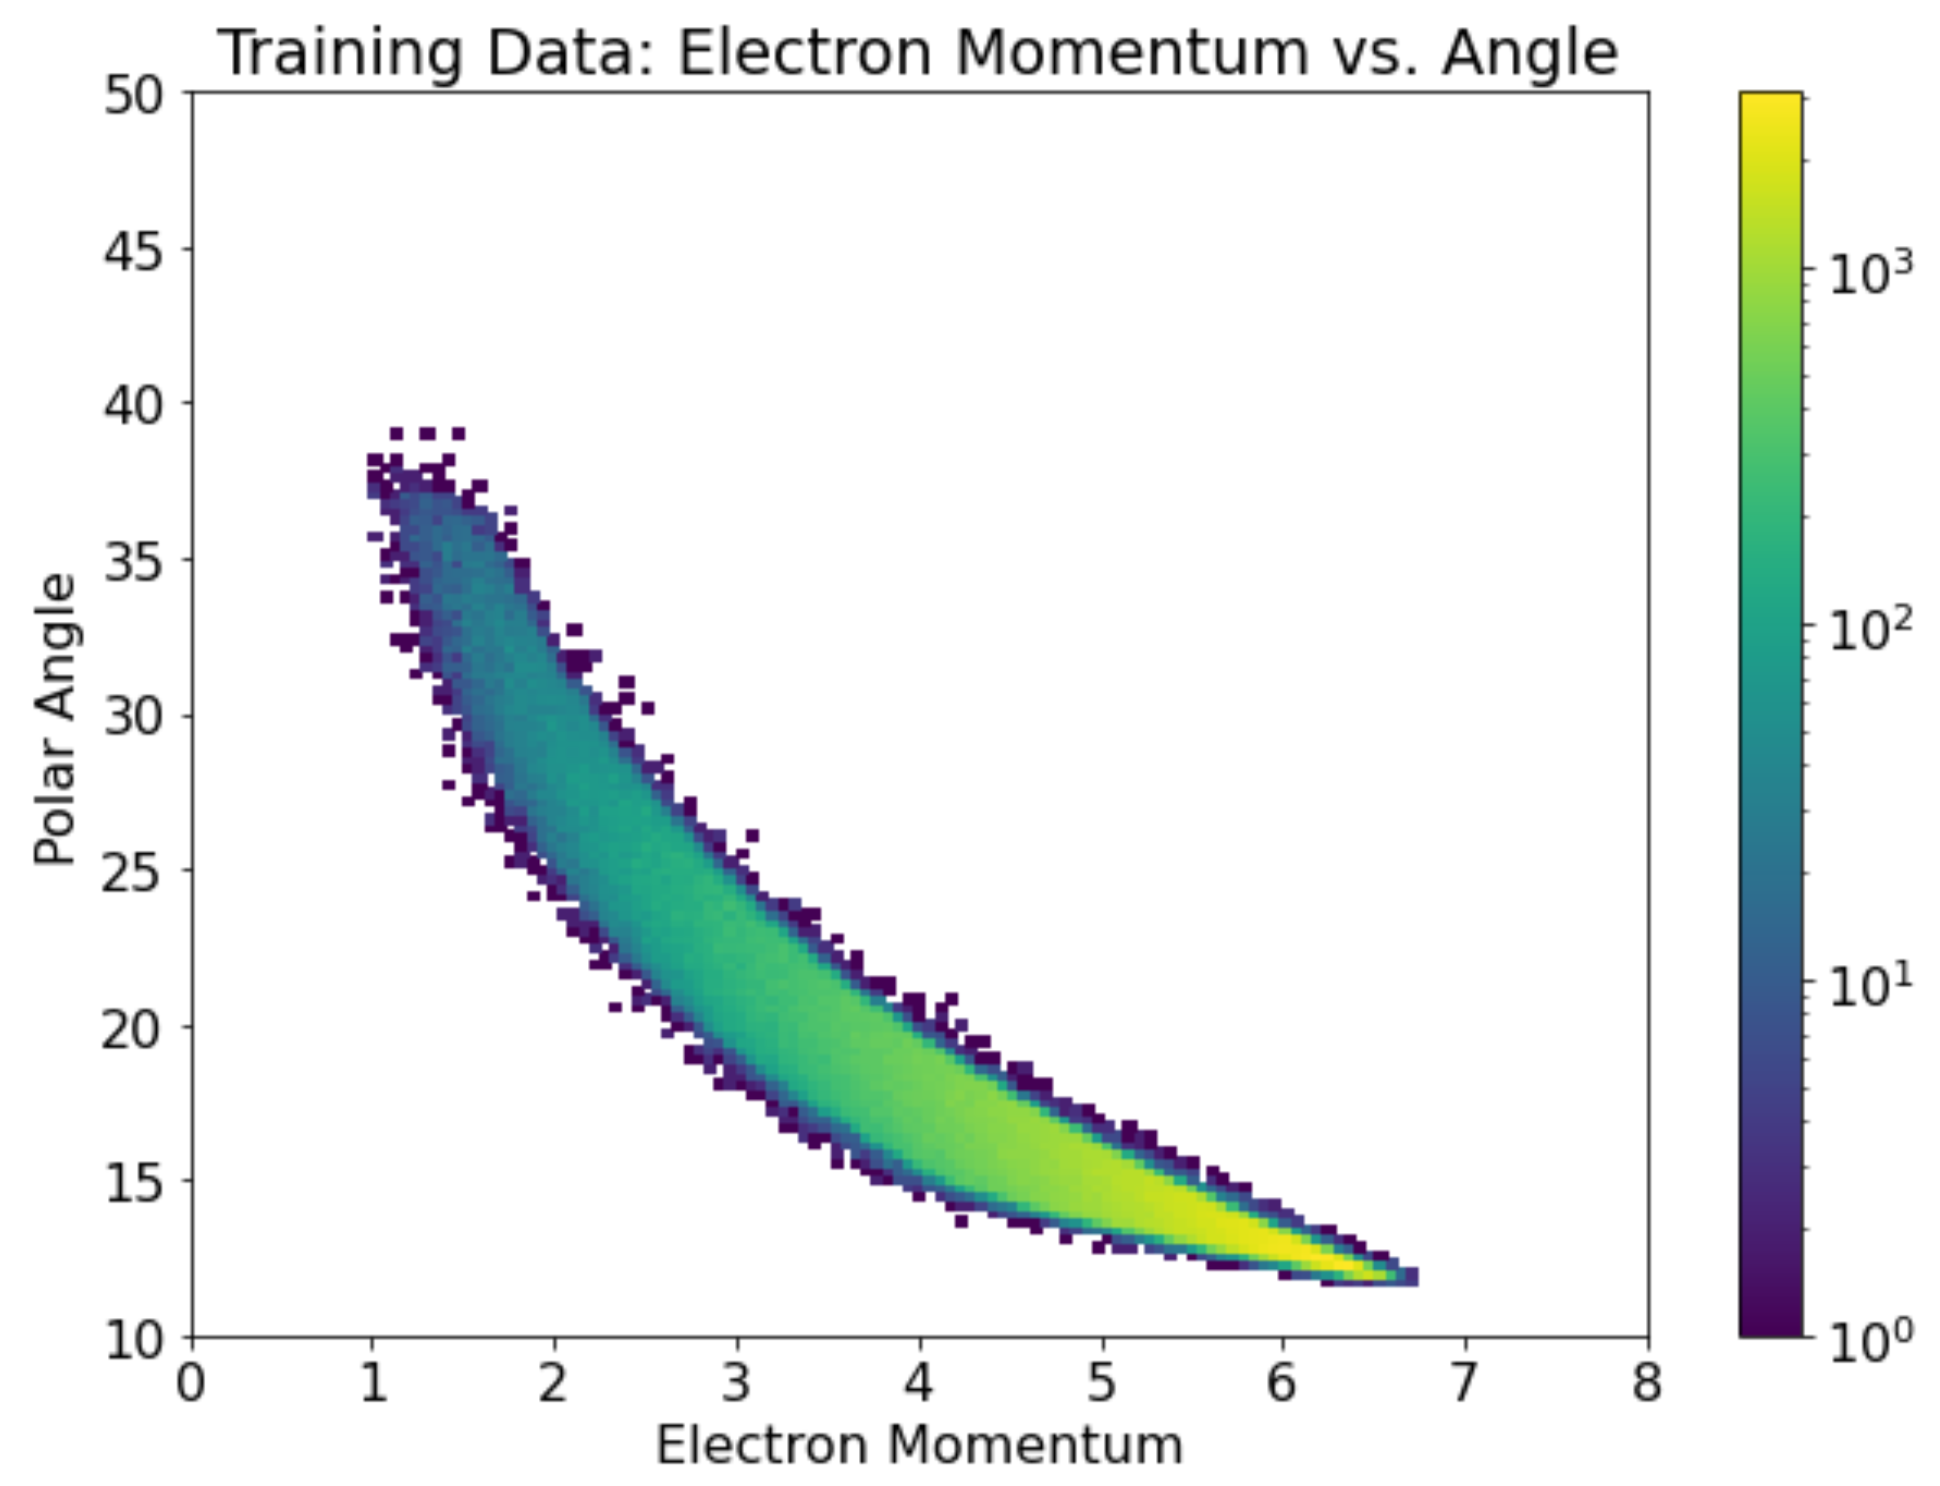
\includegraphics[width=.8\textwidth,trim={0 0 5cm 0},clip]{pictures/training_data_distribution_hires.png}
        %\caption{(a)}
        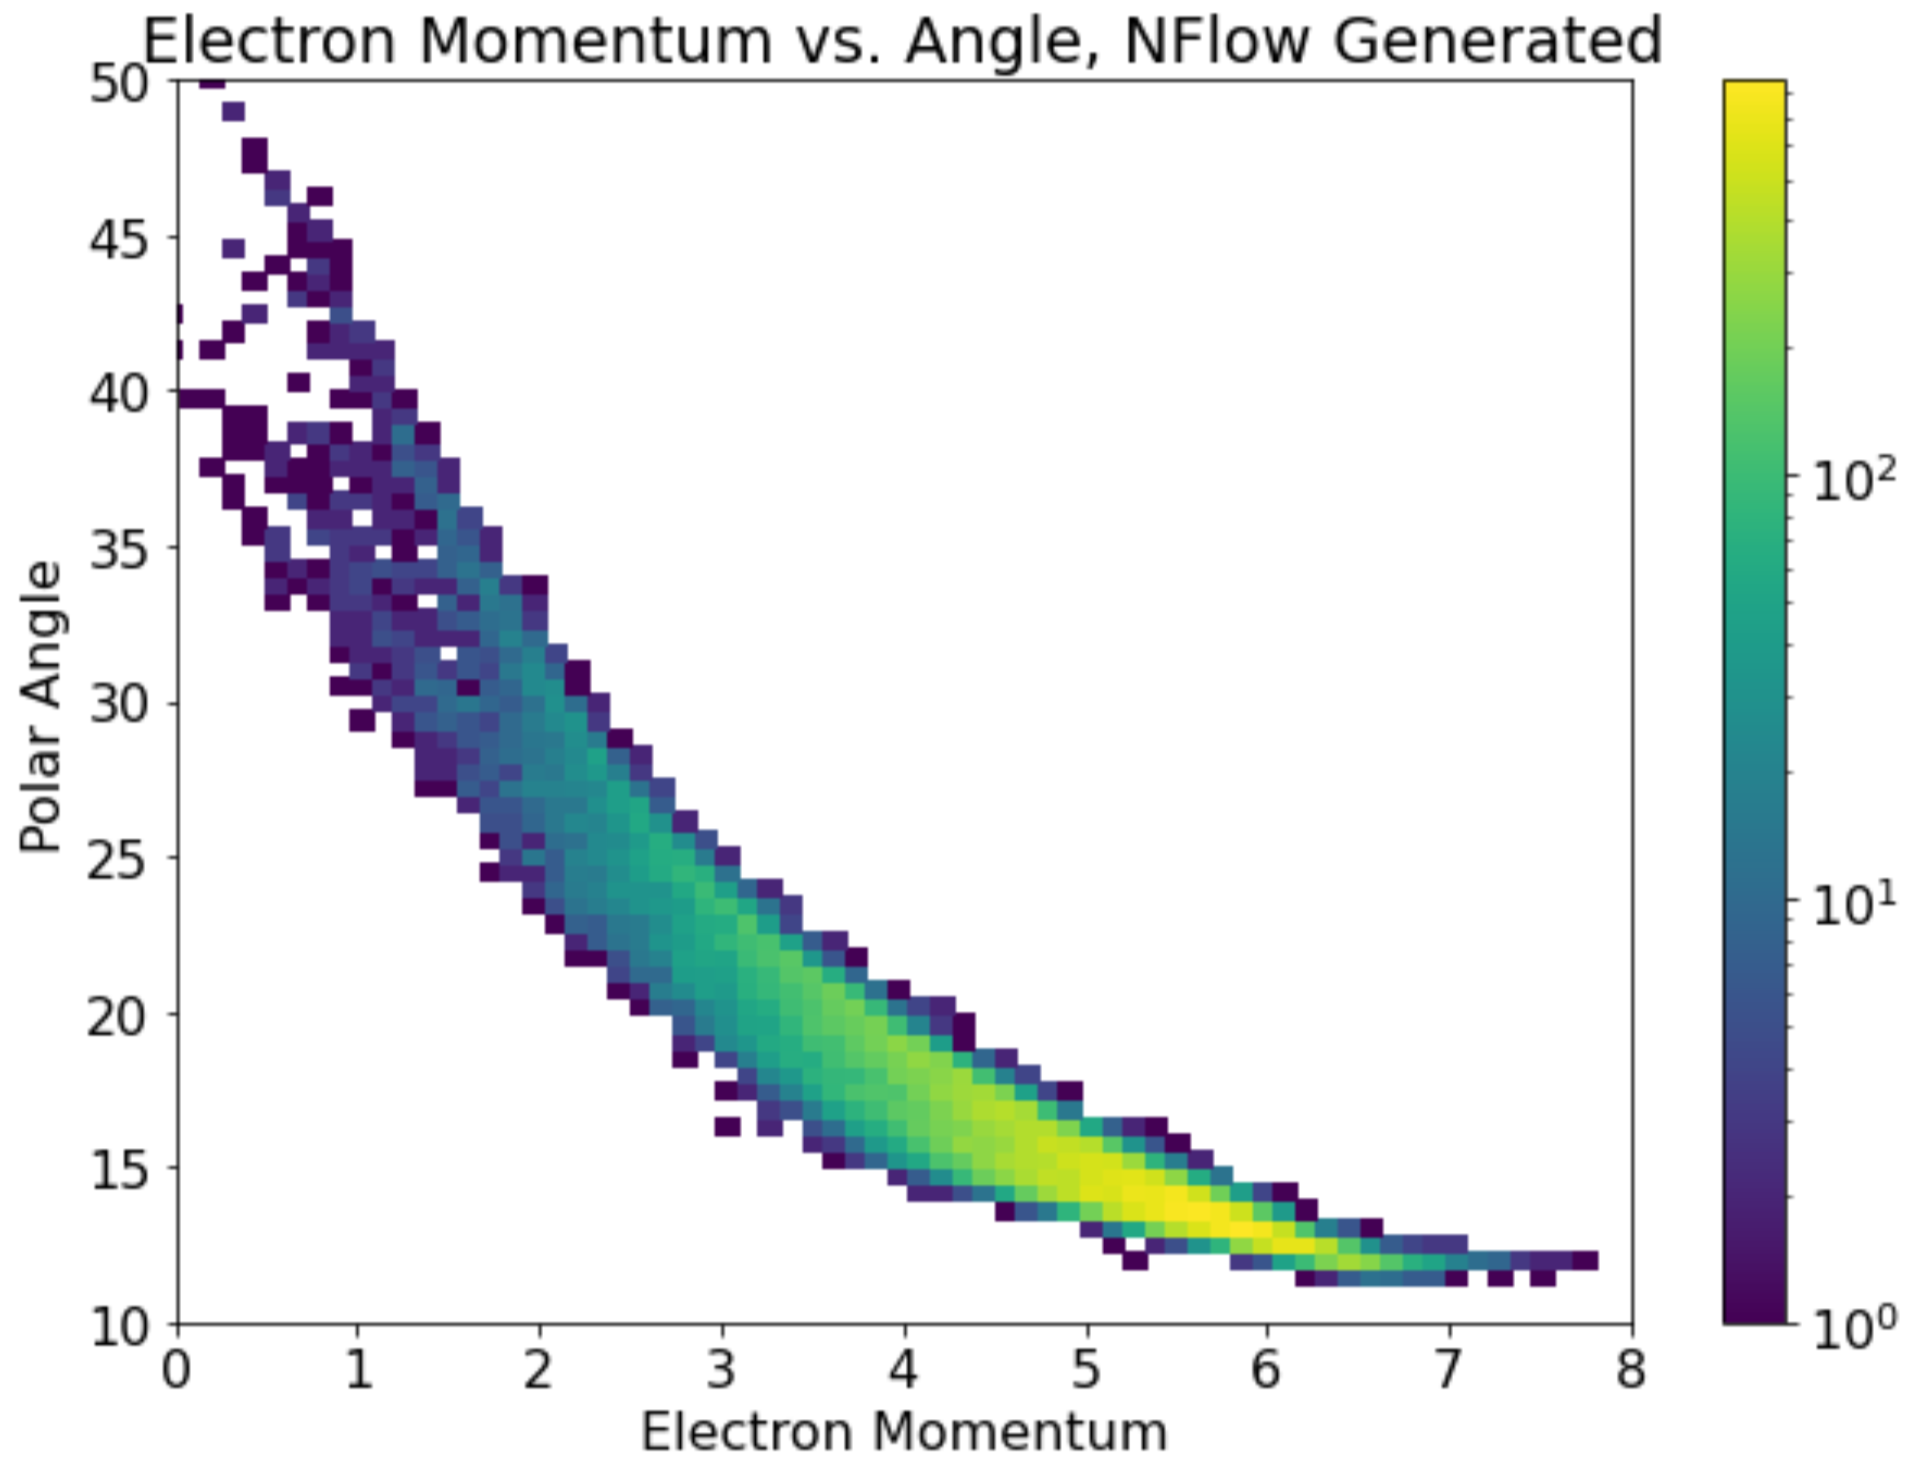
\includegraphics[width=.8\textwidth,trim={0 0 5cm 0},clip]{pictures/nflow_data_distribution_hires_0.png}
        %\caption{(c)}
    \end{minipage}%
    \begin{minipage}{0.5\textwidth}
        \centering
        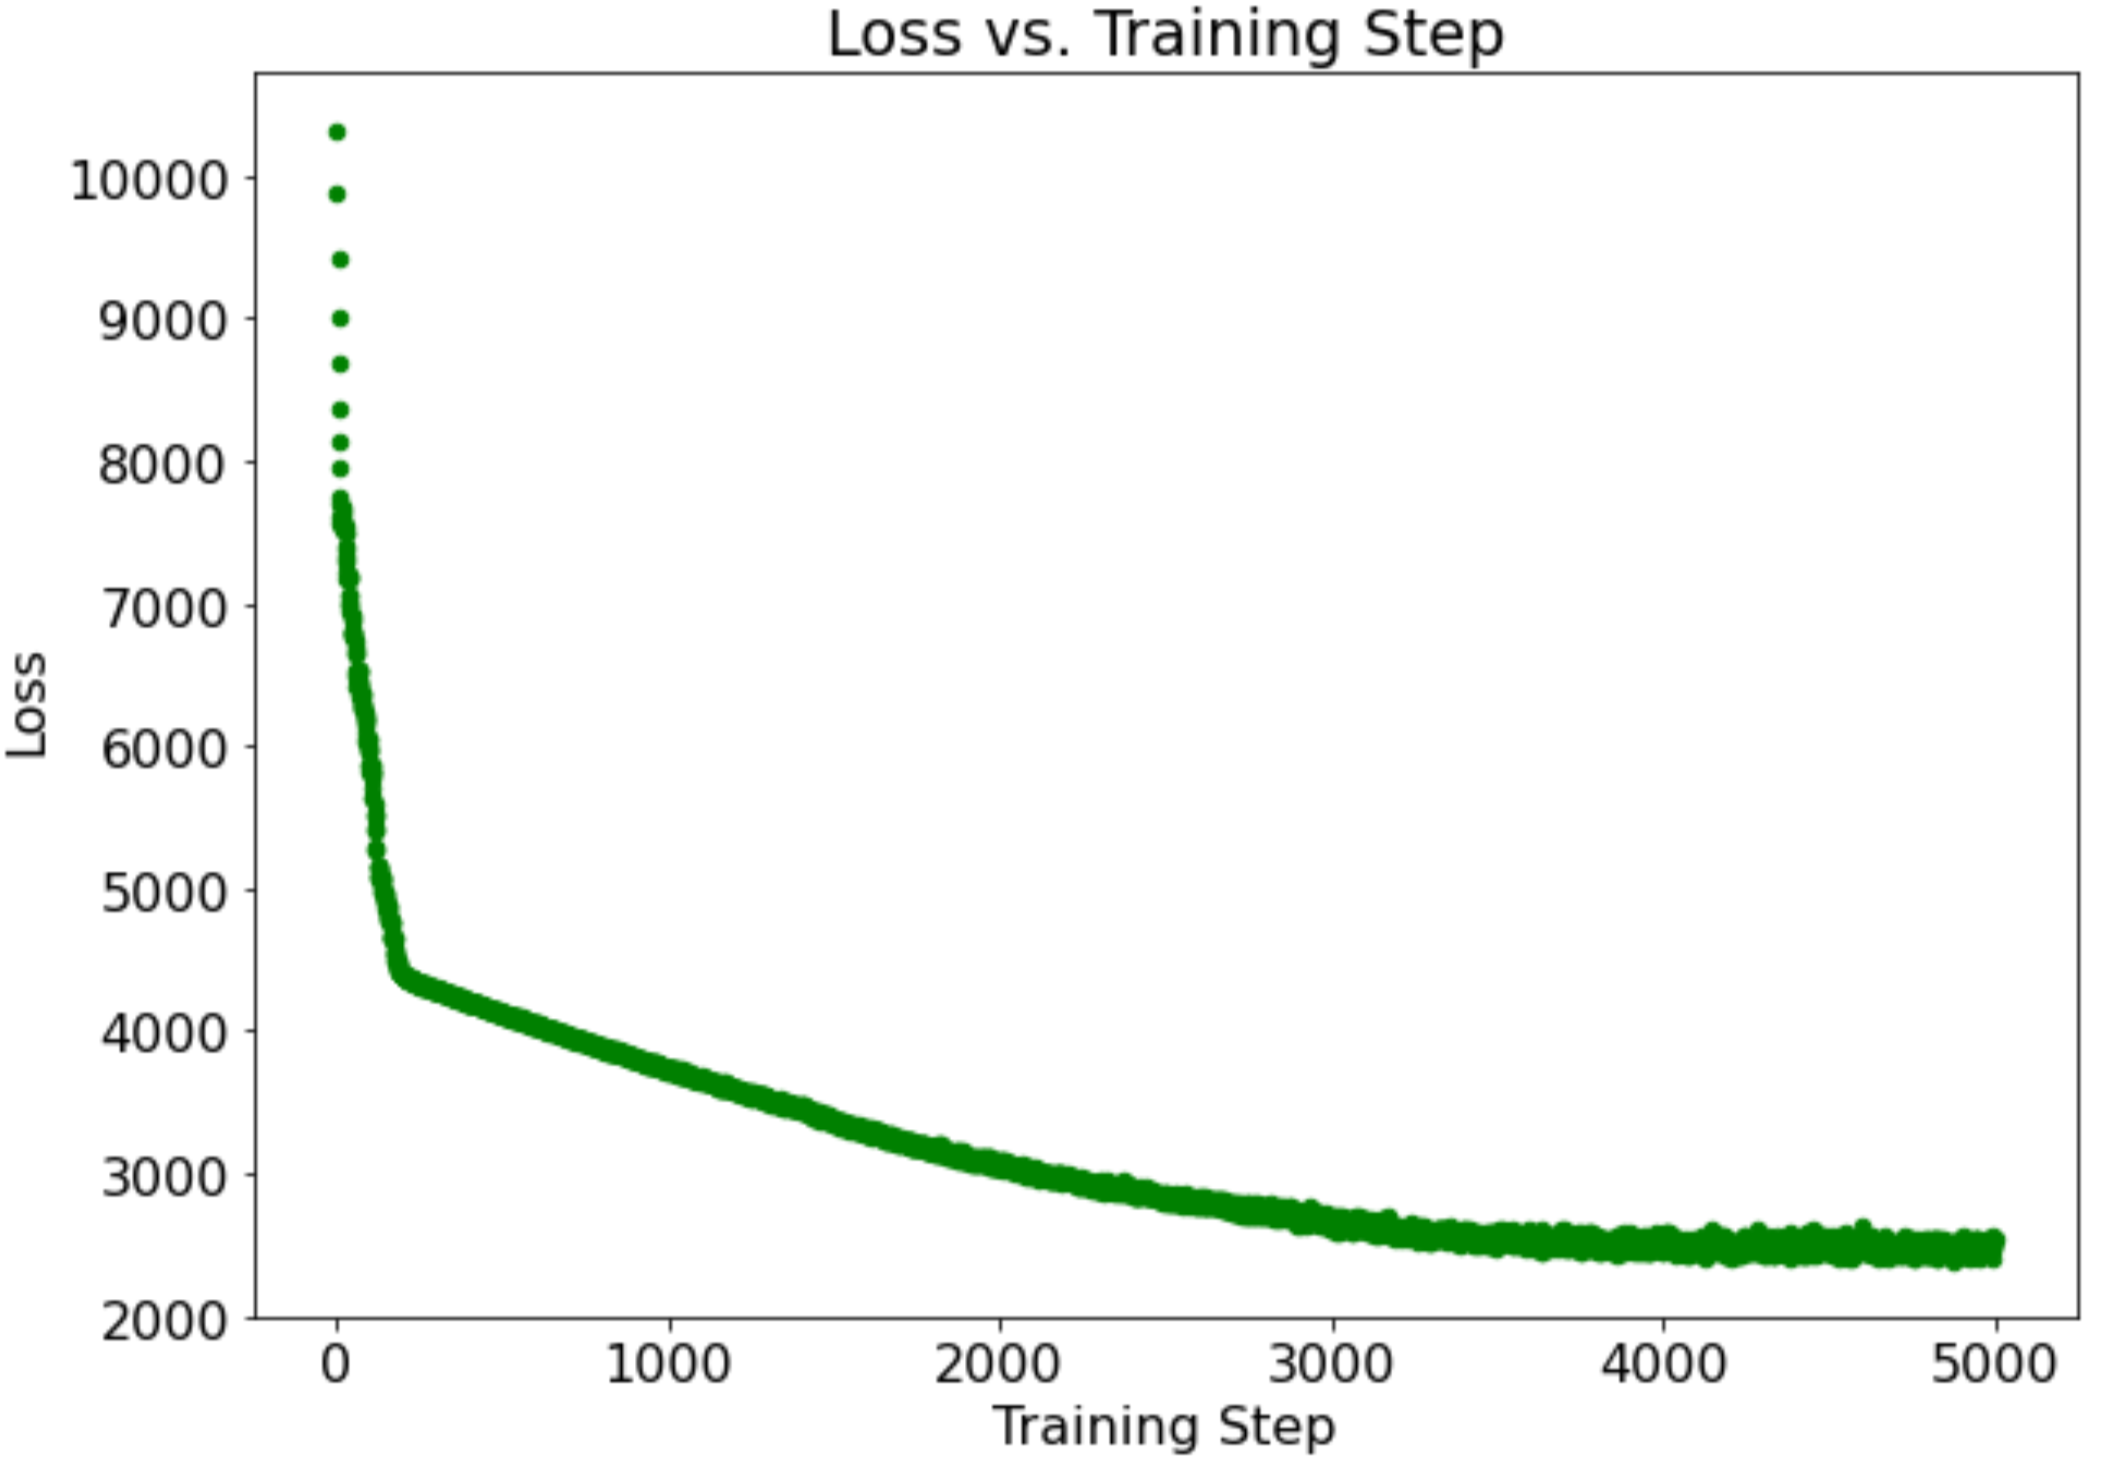
\includegraphics[width=1\textwidth,trim={0 0 0 0},clip]{pictures/loss_vs_time_2.png}
        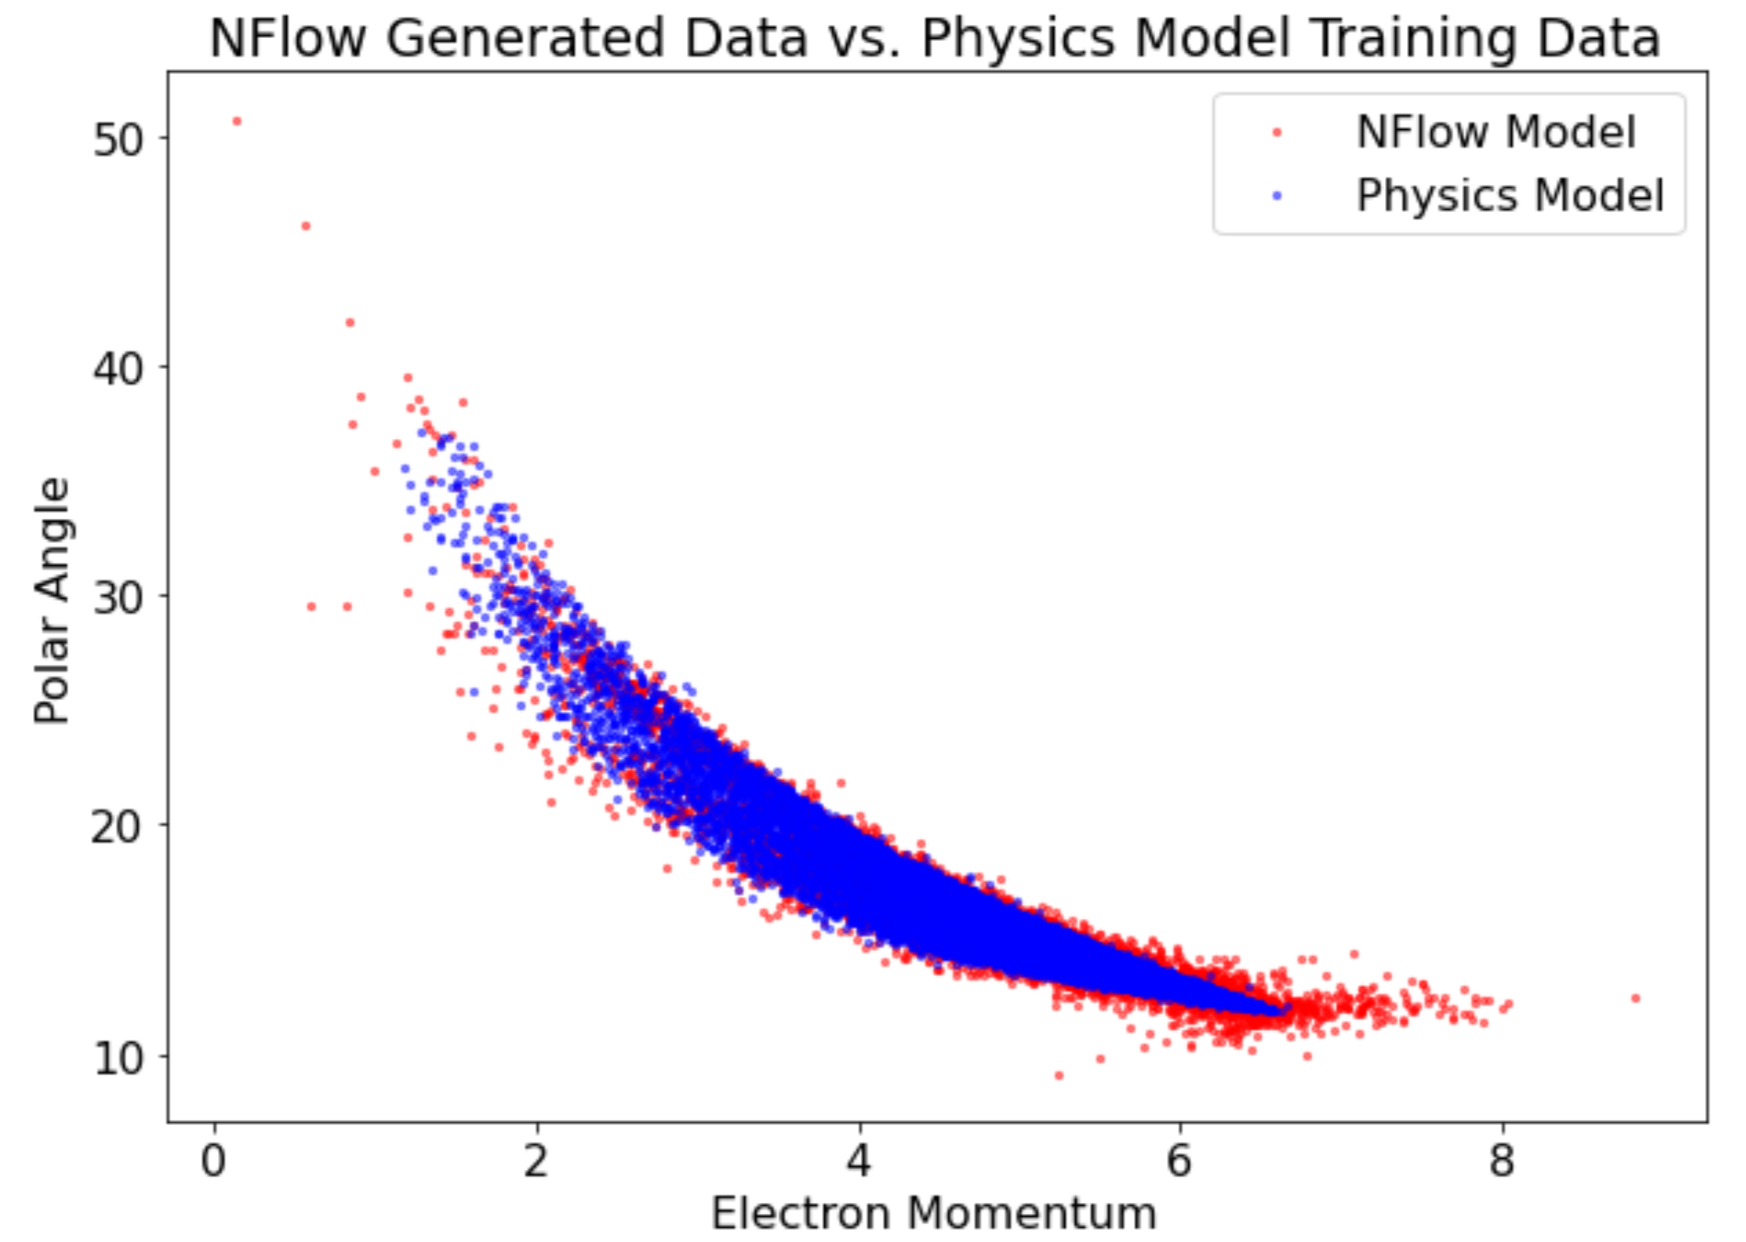
\includegraphics[width=1\textwidth,trim={0 0 0 0},clip]{pictures/nflow_vs_gemc.png}
    \end{minipage}
    \caption{Top Left: Distribution of features of training data. Top Right: Loss vs. training step. Bottom Left: Data generated from trained MAF algorithm. Bottom Right: Spatial overlay of MAF generated data and microphysics Geant4 generated data.}
    \label{fig:a}.
\end{figure}

The top right subplot of Figure \ref{fig:a} shows the training loss vs. iteration in training, from which we can see that after about 4,000 steps we converge to a minimum loss value. At this point we can use the trained model to produce data from the learned distribution, which is shown in the bottom left of Figure \ref{fig:a}.

Qualitatively, the NICE generated data is peaked around similar values, but has longer tails than the microphysics generated data. At this stage it is not clear what is causing this discrepancy, or how it can be mitigated. It is possible that including more features in training will provide higher fidelity results due to the correlations between features, but this is an active area of our research.



\iffalse
Path forward:\\
Utilization of "z" distribution to train prior distribution\\
Development and implementation of quantitative comparision methods\\
Expand to full feature representation learning\\
Move off of colab onto stronger computing platforms
\fi


\iffalse
Parameters for best run:

prior = TransformedDistribution(Uniform(torch.zeros(2), torch.ones(2)), SigmoidTransform().inv) # Logistic distribution
#prior = MultivariateNormal(torch.zeros(2), torch.eye(2))
# NICE
flows = [AffineHalfFlow(dim=2, parity=i%2, scale=False) for i in range(12)]
#print(flows)
flows.append(AffineConstantFlow(dim=2, shift=False))
#print(flows)


# construct the model
model = NormalizingFlowModel(prior, flows)

optimizer = optim.Adam(model.parameters(), lr=5e-4, weight\_decay=1e-9)
for k in range(5000):
    sampleDict = xz.sample(1000)
    

 Path forward:
 working just on google colab, we quickly run into computing performance issues
 \fi
    
%For final report
\begin{abstract}
We demonstrate a proof of principle for using a normalizing flow to learn a physics process's probability distribution in order to decrease physics simulation computing time and requirements. In this work, we used traditional physics simulations to generate a dataset $\mathbf{x}$ of 5 million data points with each data point having 16 or 4 features.  We take as input a constant 16D or 4D normal distribution $p(\mathbf{z})$, and examine whether the flow model can learn the transformation to $p(\mathbf{x})$ using a random subset of $\mathbf{x}$ for training. We observed a reasonable agreement between the results of the flow-based modeling and traditional physics methods while achieving a computational speedup factor of 10 to 1,000, but the flow is currently unable to reproduce some fine-detailed structures of the physics process.
\end{abstract}
\section{Introduction including Related Works }
%(we can now cite Stan's work! \textcolor{red}{did he already submit his thesis to DSpace MIT?})

Large scale particle physics experiments use humankind's largest machines to study nature at the smallest scales. One such experiment, called CLAS12 in Virginia at the Thomas Jefferson National Accelerator Facility (JLab) (\citet{BURKERT2020163419}), collides ultrarelativistic electrons moving only 1 m/s slower than the speed of light into an ultracold bunch of hydrogen to glean information about the substructure of the proton. In particular, two photons, one electron and one proton in the final state is known as Deeply Virtual $\pi^0$ Production (DV$\pi^0$P), and this process is currently under detailed study as its properties are related to the mechanical properties of the proton (\citet{PhysRevD.55.7114}).

The standard technique to validate experimental particle physics results is to compare real data to the output of detailed experimental simulations, wherein Monte-Carlo (MC) methods are used to walk simulated particles through a detector system in many small time steps (\citet{PhysRevLett.115.212003, 10.1093/ptep/ptaa104}). This microphysics processing begins with field-theoretic functions and empirical physics models, and swims each particle iteratively through a model geometry, solving matrices of force equations at every step. This simulation, typically performed using the GEANT4 package (\citet{AGOSTINELLI2003250}), is very computationally expensive: processing the optimal number of physics events (10,000) on a 2 GB single core takes 5 hours. Among 10,000 processed events, only about 100 events has the full final states after GEANT4 simulation mainly because of the low detecting probabilities.

Our real physics experiment will produce about 10M events, and with the common expectation of a factor of 10 more simulation data compared to real data, we will need 500M simulated physics events, which would consume 250,000 core-hours. Thus, we stand to save a huge amount of processing time if we can train a model on the distribution generated by only several million microphysics generated datapoints, and sample the rest from the trained model. Several groups in particle physics are trying to develop similar methods, for example, training flows to reduce LHC simulation time (\citet{stan}) or work at MIT's IAIFI focused on speeding up aspects of Lattice QCD by a factor of up to 1,000 (\citet{phialia}).


The normalizing flow is an effective model to learn a probability distribution $p(x)$ when a sample data set $X=\{x\}$ following the distribution is given. The basic idea is a series of transformation $g_i$'s, which are referred to as flows, transforms a prior probability $p(z)$ distributions into the target distribution $p(x)$. That is
\begin{align}
    \mathbf{x} =& g_N \circ g_{N-1}\circ ... \circ g_1 (\mathbf{z}) \\
    \mathbf{z} =& f_1 \circ ... \circ f_{N-1} \circ f_N (\mathbf{x}) \label{eqn:invertible}
\end{align}
, where $f_{N-i+1}\equiv g_i^{-1}$ following \citet{9089305}'s convention. Both $\mathbf{x}$ and $\mathbf{z}$ are vectors of the same dimension $d$. From the eq.~\ref{eqn:invertible}, $g_i$ requires an invertibility condition. An intermediate flow $\mathbf{z_i}$ is defined as follows.
\begin{align}
\mathbf{z_i} =&g_i \circ ... \circ g_1(\mathbf{z}) \label{eqn:forward}\\
    =&f_{i+1}\circ ...f_N(\mathbf{x}) \label{eqn:backward}
\end{align}
, where the flow is expressed in forward direction at eq.~\ref{eqn:forward}, and in backward direction at eq.~\ref{eqn:backward}. Therefore, $\mathbf{z_{i+1}}=g_i (\mathbf{z_i})$ and $\mathbf{z_i} = f_{N-i+1}(\mathbf{z_{i+1}})$ for one flow, or layer. If the $f_i$'s are differentiable, the PDF evolves as follows.
\begin{align}
 p(\mathbf{z_{i+1}})=& p(\mathbf{z_i})|\frac{\partial f_{N-i+1}}{\partial \mathbf{z_i}}| =p(\mathbf{z_i})|\frac{\partial g_{i}^{-1}}{\partial \mathbf{z_i}}|\\
 \log p(\mathbf{z_{i+1}}) =& \log p(\mathbf{z_i}) + \log|\frac{\partial g_i^{-1}}{\partial \mathbf{z_i}}| \label{eqn:logprob}\\
 \log p(\mathbf{x}) =& \log p(\mathbf{z}) + \sum\limits_{i=1}^N \log|\frac{\partial g_i^{-1}}{\partial \mathbf{z_i}}|.
\end{align}
Eq.~\ref{eqn:logprob} is useful to define the forward and the backward propagation of each layer.
Once the NF model is trained to learn the distribution $g: p(z)\rightarrow p(x)$, it is possible to sample $x$ using sampled $z$. \citet{PhysRevD.101.076002} showed that the Nonlinear Independent Component Estimation (NICE) (\citet{Dinh15}) implementation of NF performs well by comparing the technique to existing methods in terms of efficiencies that are defined as average weight during the generation.

Motivated by \citet{stan}'s work, we use Masked Autoregressive Flows (MAF, \citet{papamakarios2018masked}), which is one of the generalized versions of NICE. The MAF starts from a simple fact that $p(z_{i}) = \prod\limits_{j}p(z_{i,j}|\mathbf{z}_{i,0:j-1})$. The component $z_{i,j}$ is the $j$-th component of $z_i$, and the vector $\mathbf{z}_{i,0:j-1}$ is defined as $\{z_{i, 0}, ..., z_{i, j-1}\}$. The transformation is finally defined as
\begin{align}
    z_{i+1, j}=& \sigma_{i, j} z_{i, j} + \mu_{i+1, j}.
\end{align}
The moments $\mu_{i+1, j}$ and $\sigma_{i, j}$ are the mean and standard deviation of $p(z_{i+1,j}|\mathbf{z}_{i+1,0:j-1})$ ($\equiv p(z_{i+1,0})$ for $j=0$). We train the flows to learn $\mu_{i+1, j}$'s and $\sigma_{i, j}$'s, and sample $p(\mathbf{x})$. We have concluded that the Unconstrained Monotonic Neural Networks (UMNN, \citet{NEURIPS2019_2a084e55}) MAF to be suitable for this project that aims to learn noncontinuous distributions from stacked data files. \citet{NEURIPS2019_2a084e55} demonstrates that the UMNN-MAF successfully learn discontinuous distributions, and that sampling is possible even in the case that the transformation is not analytically invertible.

\citet{nflows} presents a good Github repository of how to train a NF for a 2-dimensional distribution. The libraries are very straightforward and use PyTorch. The architecture consists of the two layers of MAF and the 2D normal prior distribution. We modified the libraries as needed to suite our purpose \footnote{\url{https://github.com/6862-2021SP-team3/nflows}}.

\section{Methods}
%We should include our work of generating the data (GEMC) and processing the data (convert to root, pandas, pickle) as these are all non-trivial steps and a good "data pipeline"
The set of 5M data points were created by using the Open Science Grid (OSG) to process 2,500 core-hours of simulations. The original data format is in ROOT \cite{root}, which is a widely-used format in high energy physics written in C++. There have been improvements in python libraries like uproot \cite{uproot} that can interpret the ROOT data format. The data file has been read using uproot, and saved in pickle, a standard Python library for serializing data \footnote{\url{https://github.com/6862-2021SP-team3/hipo2pickle}}. The pickled data has 5M row, each of which contains the features of four individual particles. Each individual particle has 4 features (magnitude of momentum, polar angle, azimuthal angle), and the particle species. The particle species can be encoded into the particle's energy by utilizing special relativity. So, $\mathbf{x}$ has dimensions of $5\text{M}\times16$, where each element is just a floating point number. Training all 16 features is considerably more complex than training just 2 features, so we also used only a subset of our dataset features to train a 4 feature flow, with $\mathbf{\tilde{x}}$ of $5\text{M}\times4$ dimension to be able to compare the performance of the two models. %\sout{Our physics data set also includes $\mathbf{z}$ of the same dimensions as $\mathbf{x}$, but as sampled data points,} %\sout{not in the analytic distributions. This report only utilizes training from $\mathbf{x}$, with the utility of $\mathbf{z}$  being currently investigated.}%we didn't use $z$ 'till the end.


%\sout{A normalizing flow template repository was used as a base for our project;}%This was mentioned in the intro.
Our architecture consists of 16 layers of UMNN-MAF with 32 hidden variables per layer in the 16-feature case, and consisted of 6 layers with 80 hidden variables per layer in the 4-feature case. After many trials of different combinations of hyper parameters and flow models, we found that an effective training method to use 10000 epochs with each iteration using randomly sampled training data sets of 400$\times$16 dimension from the initial 5M data points generated by physics simulations. To evaluate our model, we sampled 100k data points, $\mathbf{x_1}$, from the physics simulation set which were not included in training, and generated 100k data points, $\mathbf{x_2}$, using our trained model.The Earth Mover's Distance (EMD), calculable as the Wasserstein-1 Distance (\citet{Dobrushin} was evaluate between $\mathbf{x_1}$ and $\mathbf{x_2}$. Since our sample data size was somewhat small, we sampled a second set of 100k data points, $\mathbf{x_1'}$, from the physics simulation set, and calculated EMD values between  $\mathbf{x_1}$ and $\mathbf{x_1'}$, to have a benchmark to compare with the metrics from the normalized flow comparison.


\section{Results and Discussion}
\subsection{Results from 16-Feature Trained NF Model}
Training the NF models was relatively fast, for the 16-feature model taking about 1 hour on a GPU (NVIDIA Quadro RTX 5000) or about 10 hours on a CPU (Intel Xeon E-2276M). On the other hand, sampling from the trained model was considerably slower; the 16-feature trained NF model generated datapoints at a rate of about 4 Hz, which is only a factor of 10 times faster than the traditional method of simulating the processes' microphysics. \citet{NEURIPS2019_2a084e55} and \citet{papamakarios2018masked} explains this behavior as follows. The Masked Autoencoder for Distribution Estimation (MADE, \citet{pmlr-v37-germain15}), which is a building block of MAF allows the training to be done in parallel using GPUs. Sampling data points from the trained MAF takes significant amount of time because the model requires $\mathbf{z}_{i,0:j-1}$ to sample $\mathbf{z}_{i,j}$. There is a computational trade-off in Inverse Autoregressive Flow (IAF, \citet{NIPS2016_ddeebdee}, which trains the model slowly but samples fast. Despite this known drawback, we still consider the UMNN-MAF to be the optimal model for this project because training the model to sample data points following distributions reasonably close to that of physics simulation. Figure \ref{fig:16features} shows the feature distributions of samples from this trained model, with each plot also showing the Earth Mover's Distance between the NF model data, and sample data from the microphysics distribution.


In general, the 16-feature trained NF model produces similar results to the traditional simulation's distribution, but fine details were difficult to reproduce. In particular, hard distribution cutoffs that exist in the traditional distribution due to the enforcement of conservation laws and the physics detector edges were not well learned by the NF model, while smoother distributions were reproduced well.

For a quantitative comparison, Figure \ref{fig:EMD} shows the Earth Mover's Distance between samples from the trained NF model and the traditional physics distribution. In the limit of identical distributions with infinitely many samples, the EMD is zero. Since we are working with only 100K datapoints, rather than report the EMD values by themselves (which can be seen in Figure \ref{fig:16features}), we took the ratio of the NF model - traditional physics distribution EMD value to the EMD value calculated between two sets of 100K datapoints taken from the traditional physics distribution, which had values on the order of 0.005. Thus, a perfectly trained NF model would have an EMD ratio of 1, and as we deviate above 1, we exhibit worse performance. We can see in Figure \ref{fig:EMD} that most features have a ratio of about 3--8, which is not perfect, but demonstrates reasonable agreement in line with what is observed in Figure \ref{fig:16features}. Unfortunately, we do not have the reference of these ratios to define the good sampling.

\begin{figure}[!h]
    \centering
    \begin{minipage}{.23\textwidth}
    
        \centering
       % Electron
        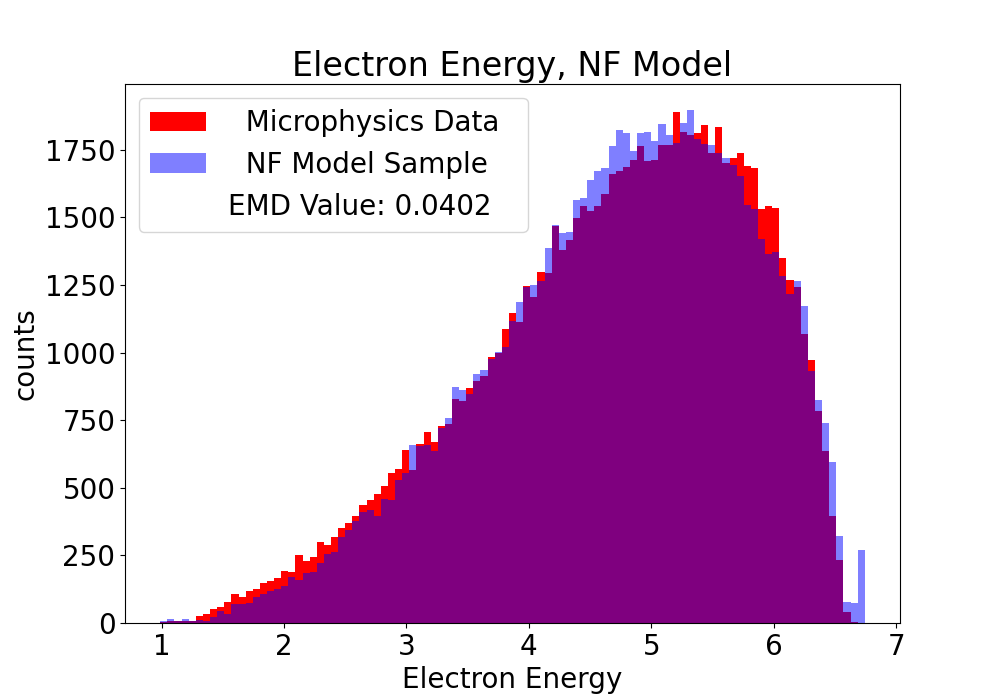
\includegraphics[width=.99\textwidth,trim={3cm 0 0 0},clip]{FinalPictures/Features16/Electron_Energy,_NF_Model.png}
        %\caption{(a)}
        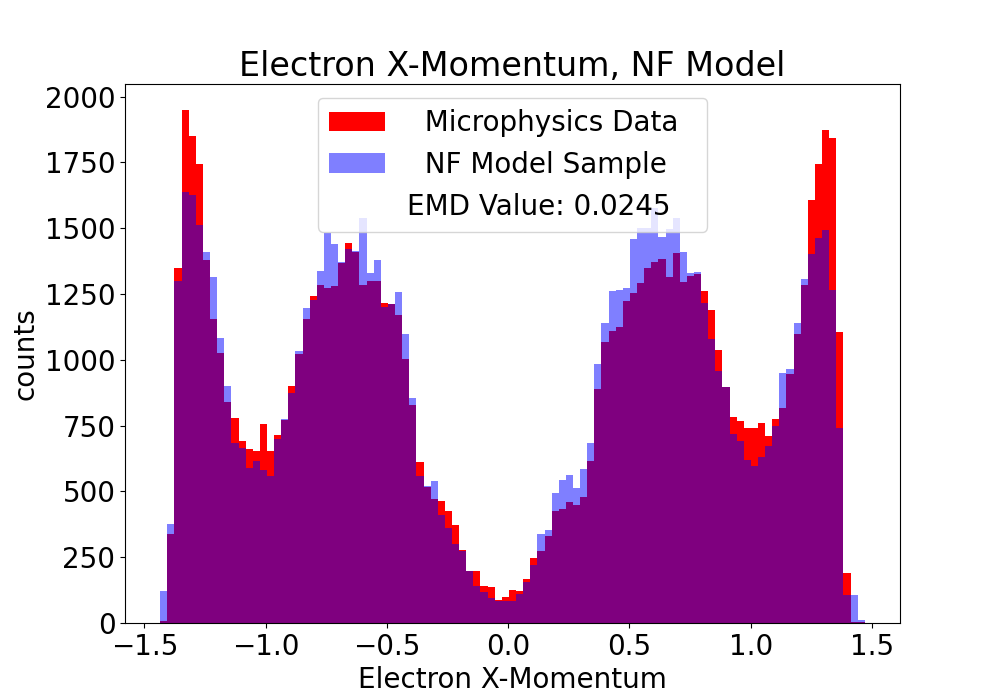
\includegraphics[width=.99\textwidth,trim={3cm 0 0 0},clip]{FinalPictures/Features16/Electron_X-Momentum,_NF_Model.png}
        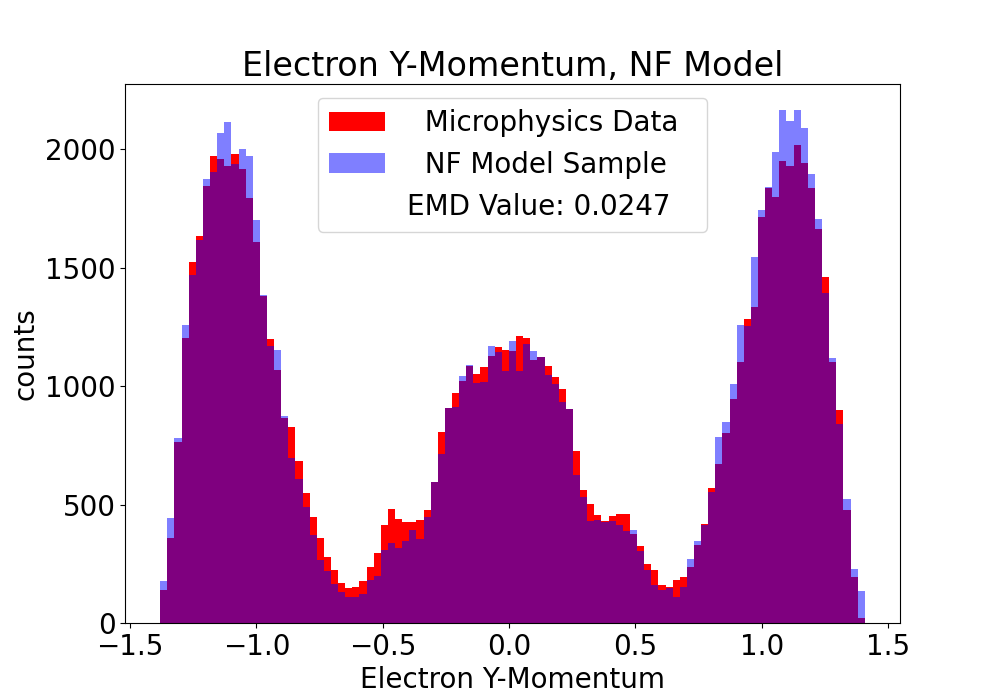
\includegraphics[width=.99\textwidth,trim={3cm 0 0 0},clip]{FinalPictures/Features16/Electron_Y-Momentum,_NF_Model.png}
        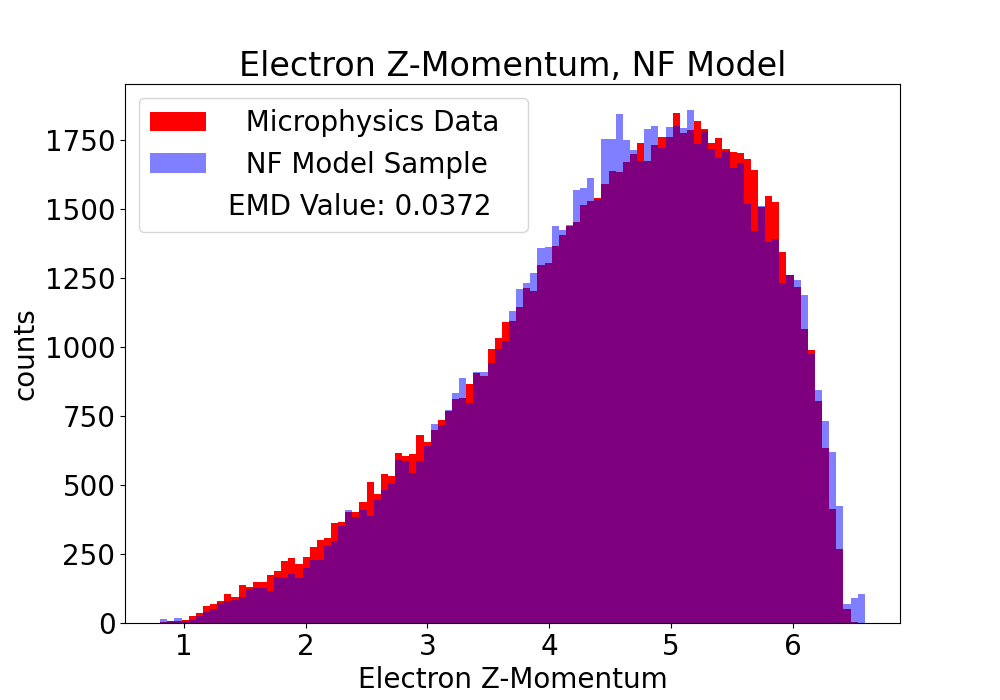
\includegraphics[width=.99\textwidth,trim={3cm 0 0 0},clip]{FinalPictures/Features16/Electron_Z-Momentum,_NF_Model.png}
        %\caption{(c)}
    \end{minipage}%
    \begin{minipage}{0.23\textwidth}
        \centering
       % Proton
        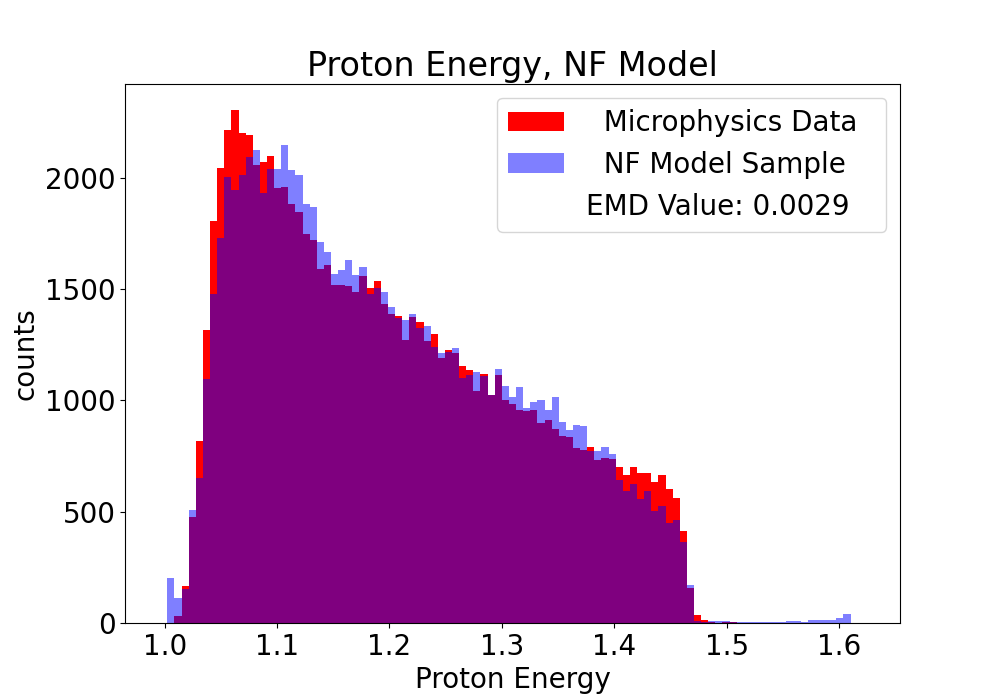
\includegraphics[width=.99\textwidth,trim={3cm 0 0 0},clip]{FinalPictures/Features16/Proton_Energy,_NF_Model.png}
        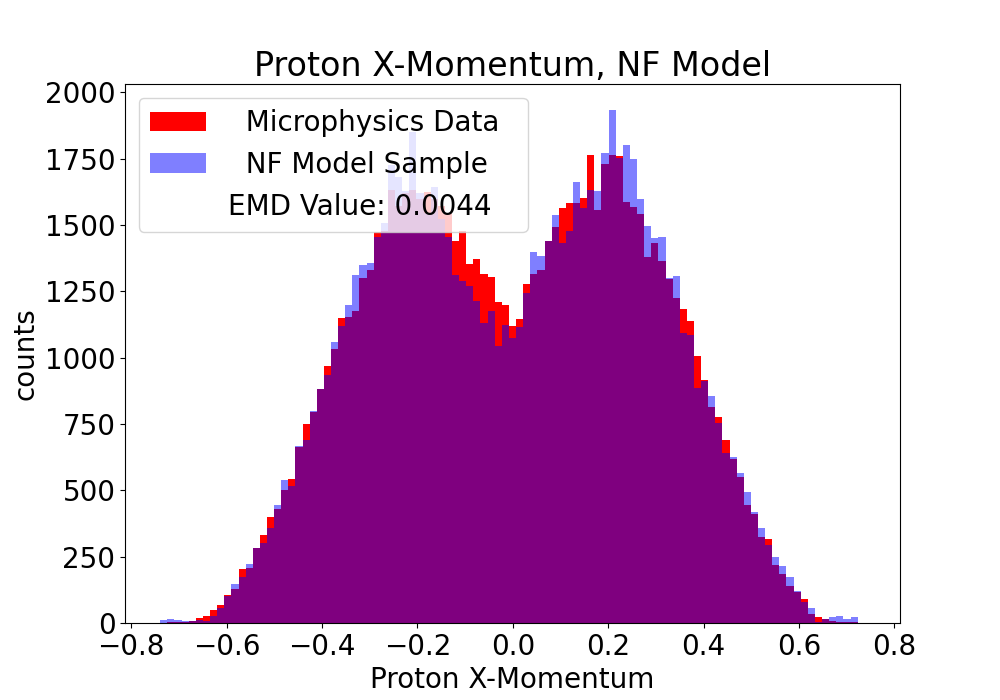
\includegraphics[width=.99\textwidth,trim={3cm 0 0 0},clip]{FinalPictures/Features16/Proton_X-Momentum,_NF_Model.png}
        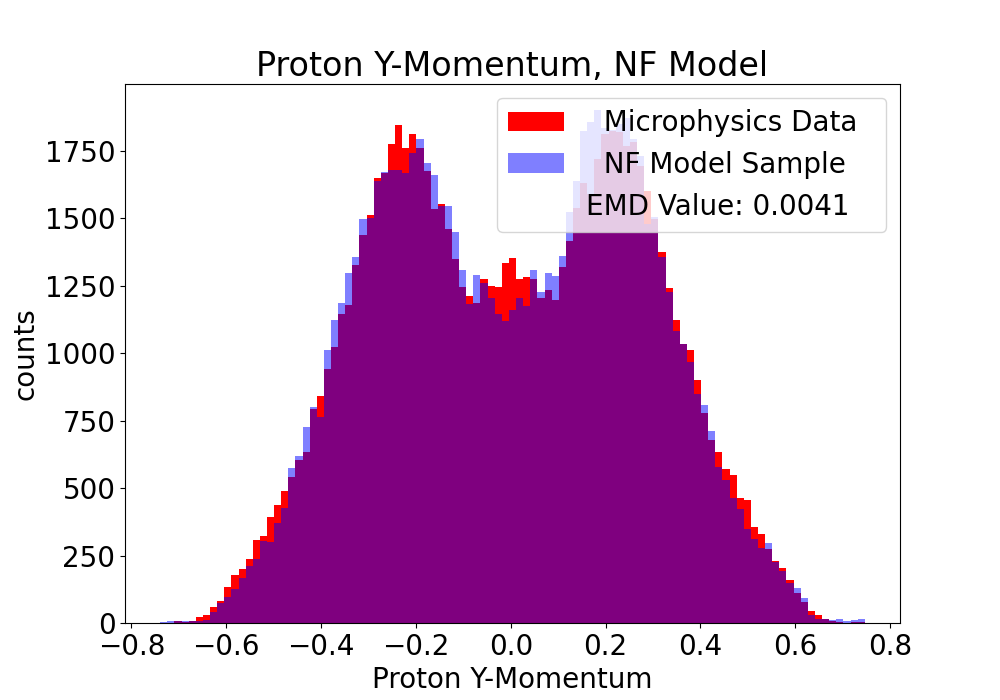
\includegraphics[width=.99\textwidth,trim={3cm 0 0 0},clip]{FinalPictures/Features16/Proton_Y-Momentum,_NF_Model.png}
        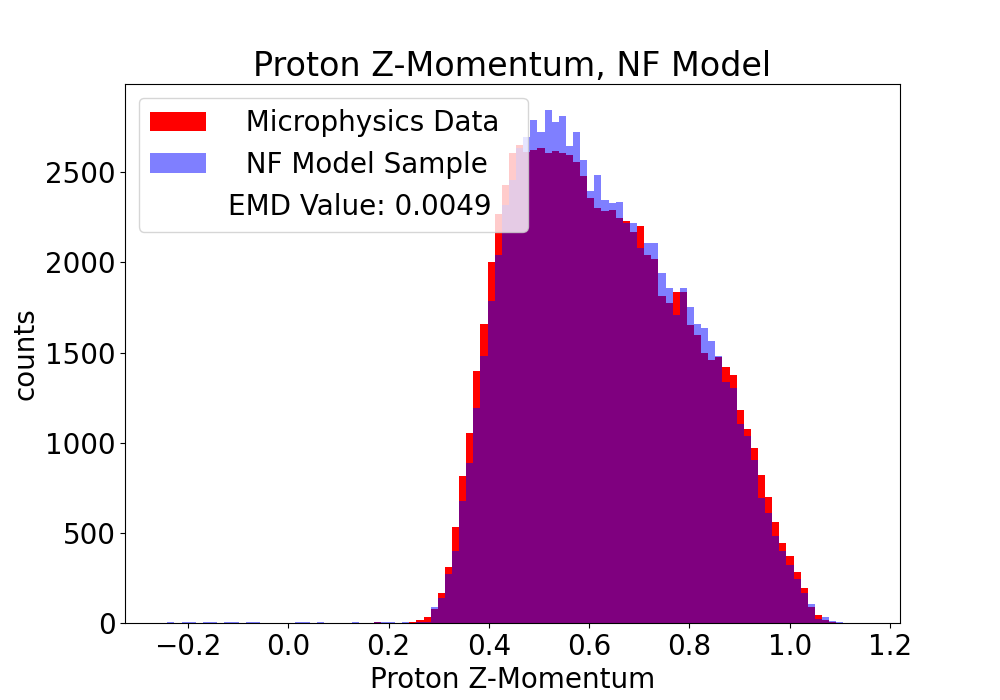
\includegraphics[width=.99\textwidth,trim={3cm 0 0 0},clip]{FinalPictures/Features16/Proton_Z-Momentum,_NF_Model.png}
    \end{minipage}
     \begin{minipage}{0.23\textwidth}
            \centering
           % Photon 1
            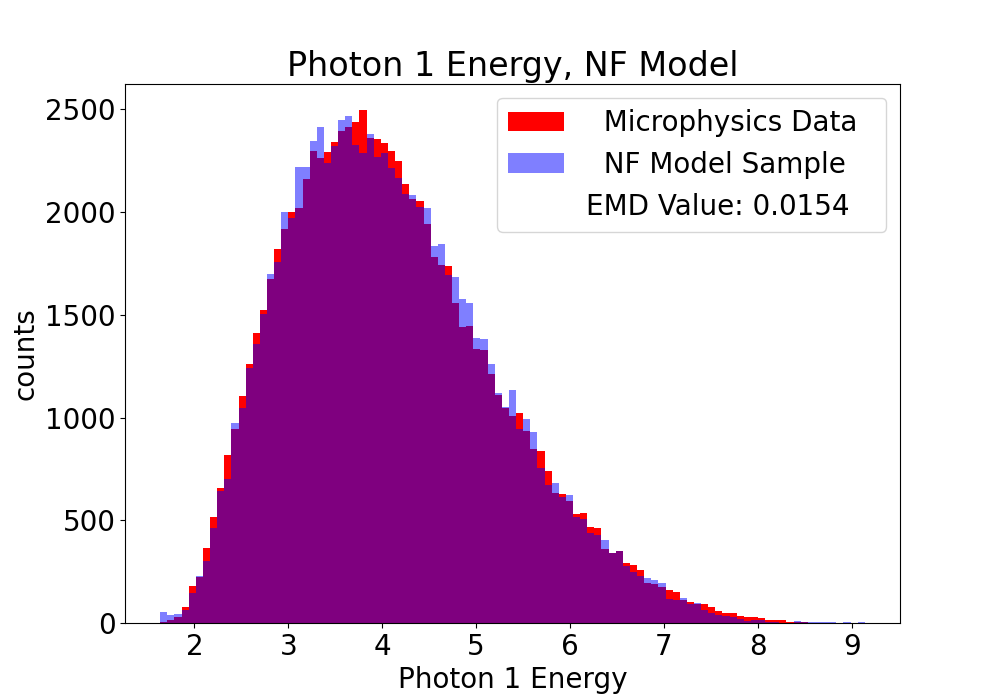
\includegraphics[width=.99\textwidth,trim={3cm 0 0 0},clip]{FinalPictures/Features16/Photon_1_Energy,_NF_Model.png}
            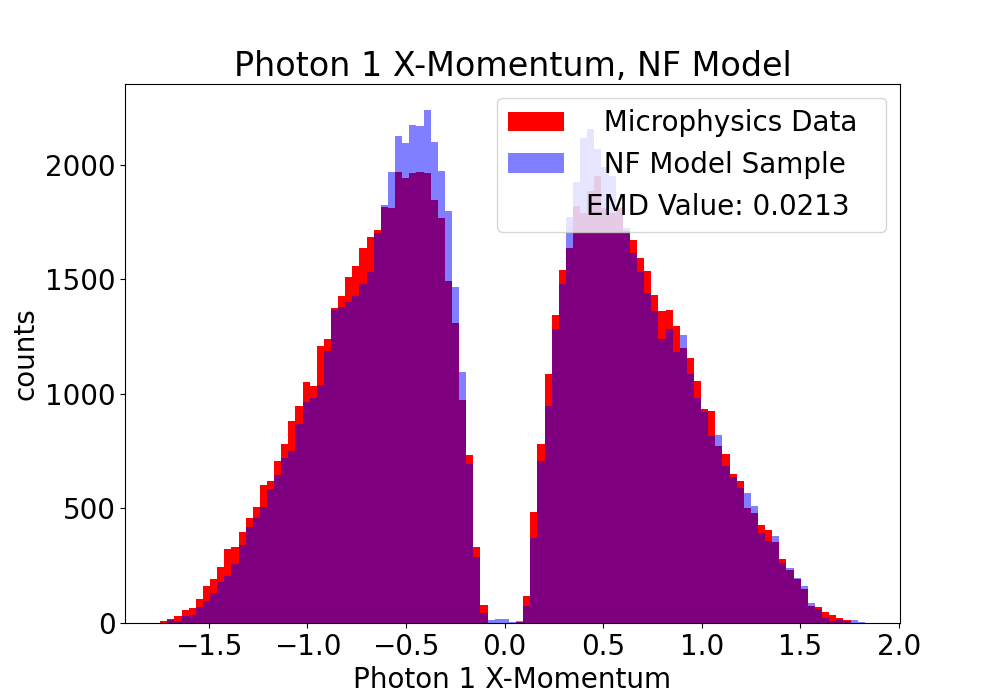
\includegraphics[width=.99\textwidth,trim={3cm 0 0 0},clip]{FinalPictures/Features16/Photon_1_X-Momentum,_NF_Model.png}
            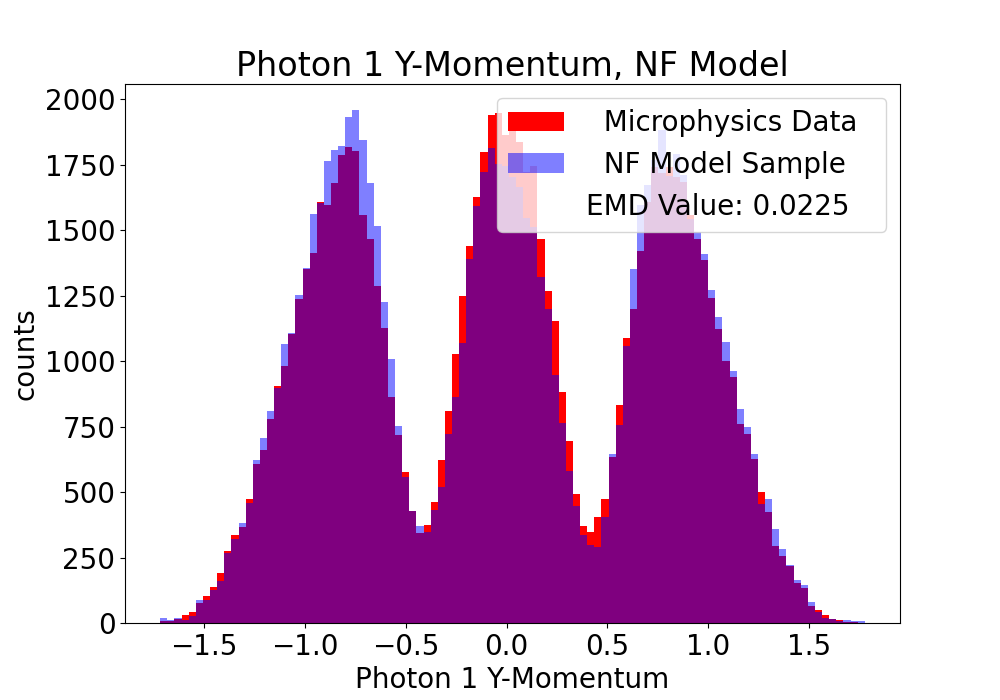
\includegraphics[width=.99\textwidth,trim={3cm 0 0 0},clip]{FinalPictures/Features16/Photon_1_Y-Momentum,_NF_Model.png}
            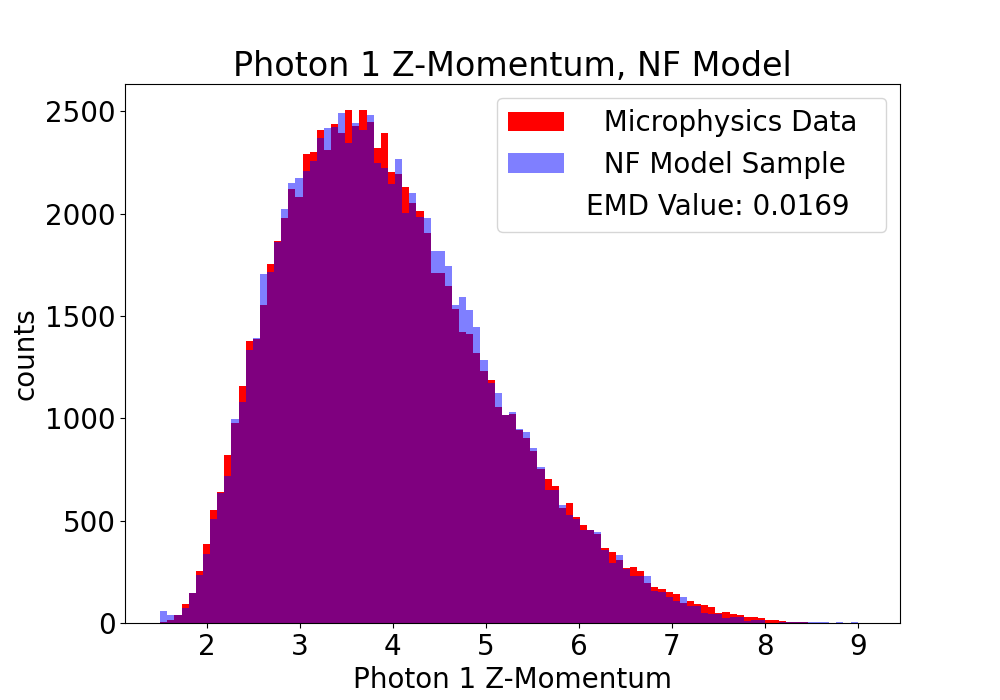
\includegraphics[width=.99\textwidth,trim={3cm 0 0 0},clip]{FinalPictures/Features16/Photon_1_Z-Momentum,_NF_Model.png}
    \end{minipage}
     \begin{minipage}{0.23\textwidth}
        \centering
        %Photon 2
        
        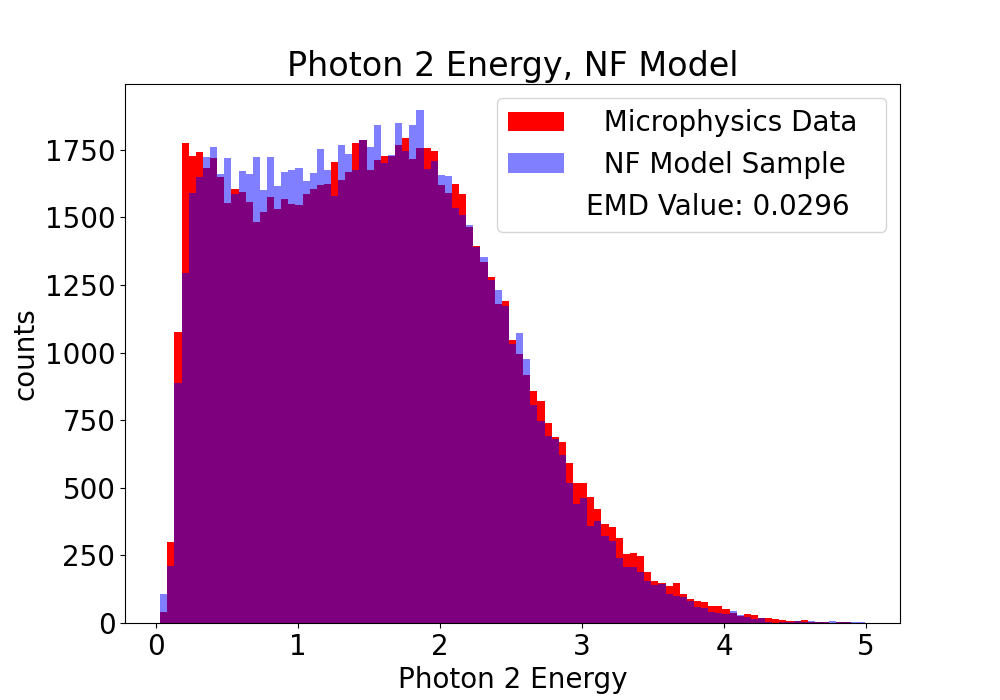
\includegraphics[width=.99\textwidth,trim={3cm 0 0 0},clip]{FinalPictures/Features16/Photon_2_Energy,_NF_Model.png}
        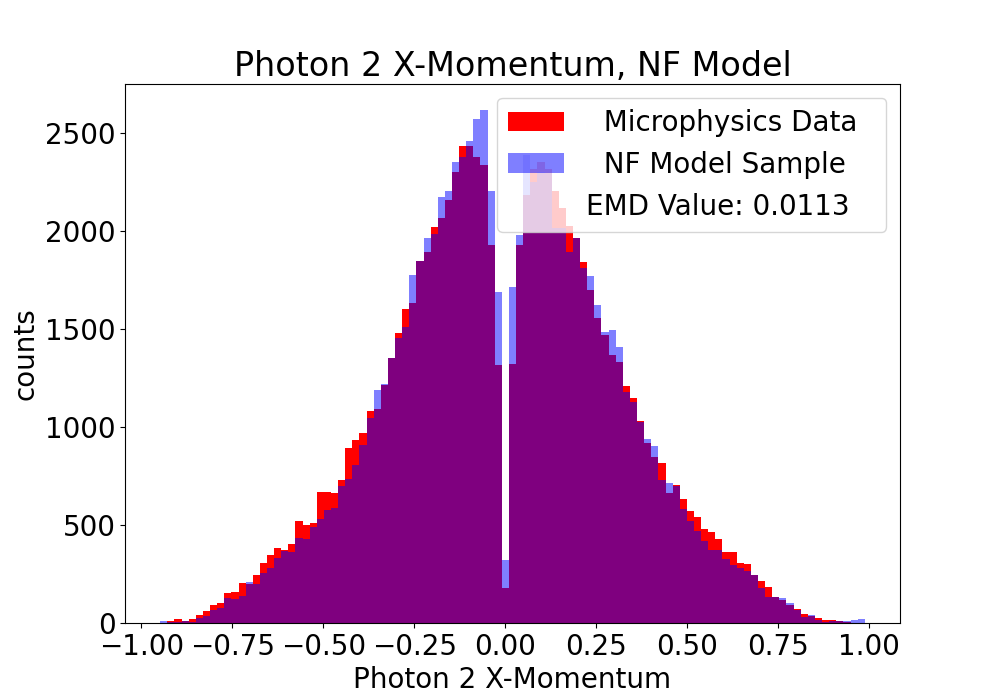
\includegraphics[width=.99\textwidth,trim={3cm 0 0 0},clip]{FinalPictures/Features16/Photon_2_X-Momentum,_NF_Model.png}
        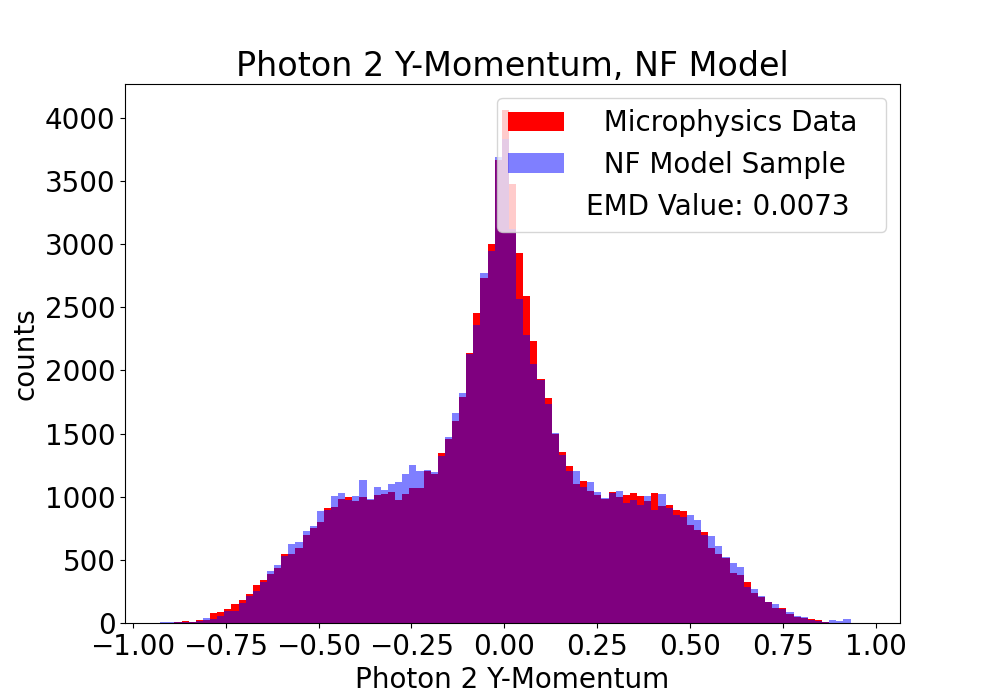
\includegraphics[width=.99\textwidth,trim={3cm 0 0 0},clip]{FinalPictures/Features16/Photon_2_Y-Momentum,_NF_Model.png}
        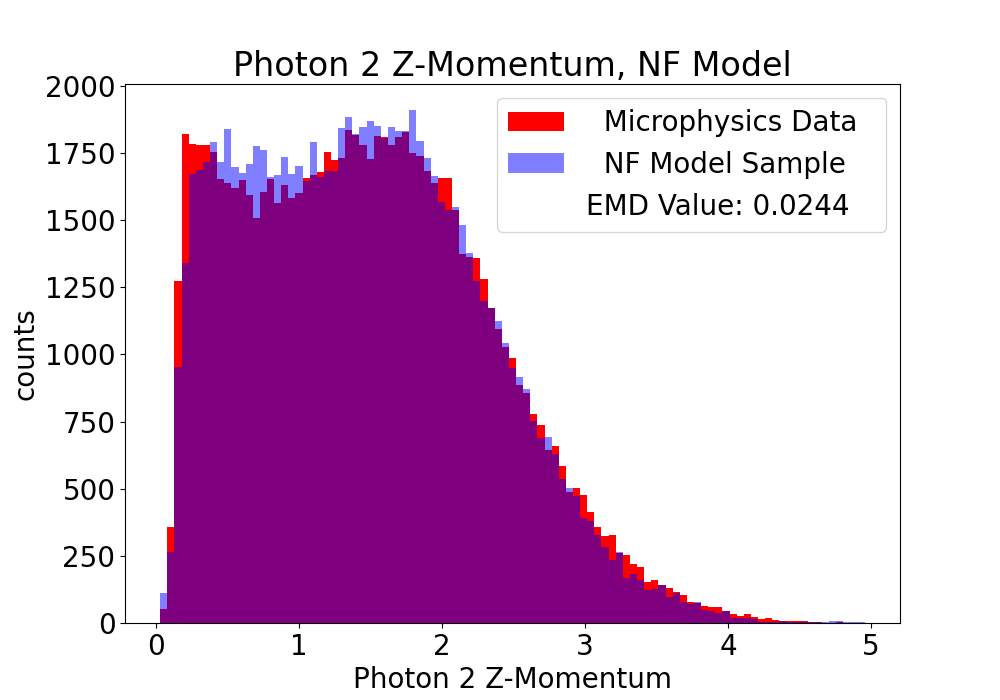
\includegraphics[width=.99\textwidth,trim={3cm 0 0 0},clip]{FinalPictures/Features16/Photon_2_Z-Momentum,_NF_Model.png}
    \end{minipage}
    \caption{The 1D distributions of all 16 features sampled from our NF model (blue), and from physics simulation (red). Each histogram is normalized to the area, and has 100 bins.}
    \label{fig:16features}
\end{figure}



\begin{figure}[!h]
    \centering
    %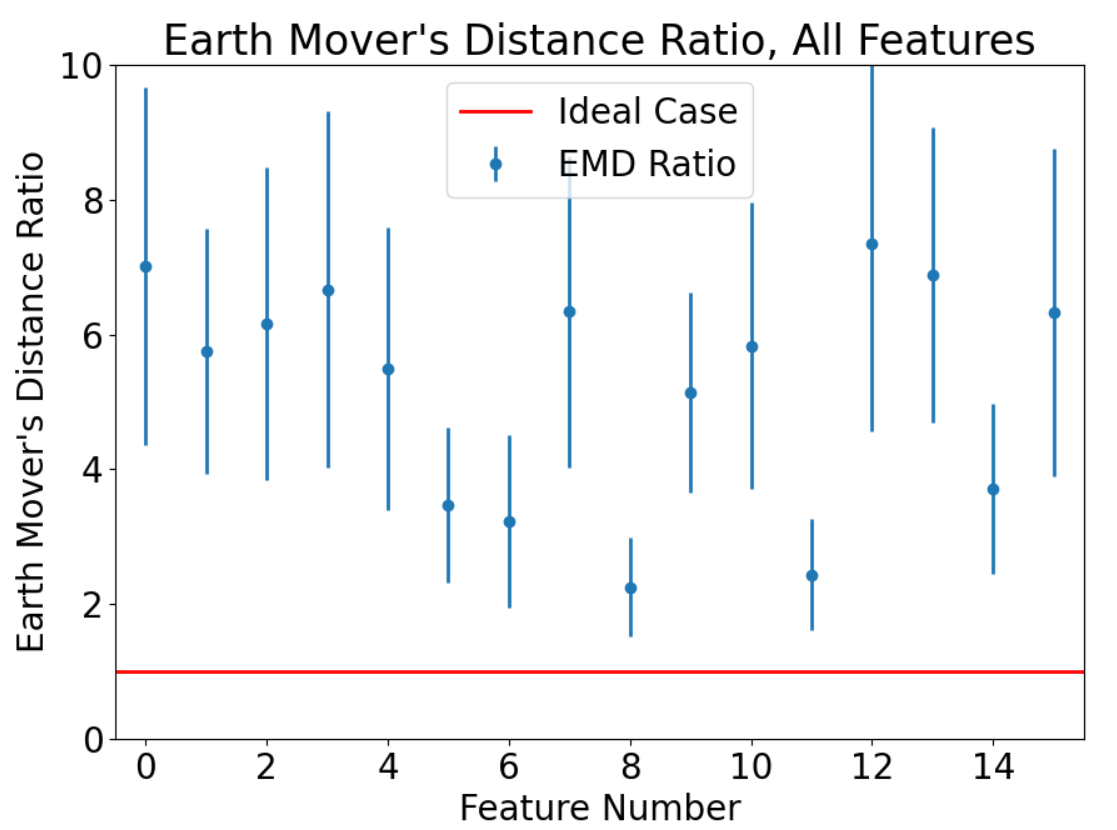
\includegraphics[scale=0.3]{FinalPictures/EMD/EmdRatio.png}
    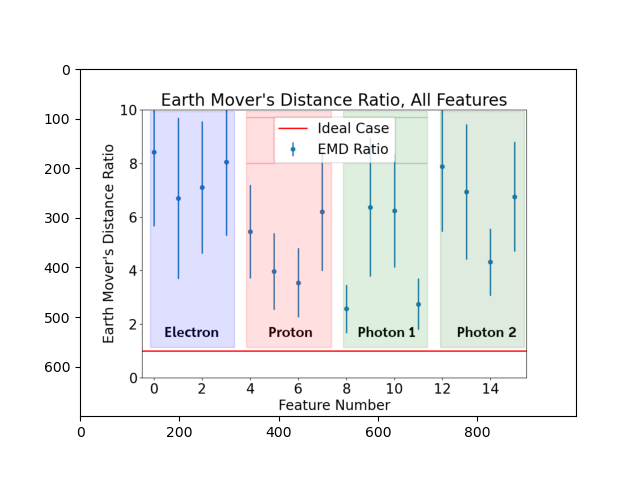
\includegraphics[width=.7\textwidth,trim={2.5cm 1.75cm 2cm 2.1cm},clip]{FinalPictures/EMD/nflow_emd_with_text.png}
    \caption{The EMD ratios of all 16 features between the NF generated distributions and sample from physics simulation. The points are the average EMD ratios of 10 different subsample calculations; the error bars are the standard deviation of the set. If the model were perfect, all points would have value 1; deviation from 1 indicates worse performance.}
    \label{fig:EMD}
\end{figure}

To understand the shortcomings of the trained model, we consider 2-Dimensional distributions in  Figure \ref{fig:2D}. We can see that while some distributions are reproduced well, the fine detail and hard cutoffs that exist in some feature spaces are not learned sharply by the model and result in haziness. Specifically, only certain combinations of particle momenta are measurable due to the physical limitations of our real-world detectors (and hence, our computer-modeled detectors in the traditional microphysics simulations) as well as due to physics conservation law constraints. However, we have yet to incorporate these constraints into our NF model training, and so the samples generated from this trained model exist in traditionally empty regions of phase space. One solution to this issue is to implement filtering after sampling from the model, but given the already slow sampling rate, this would further decrease the speed advantage offered by the normalizing flow method. Work is ongoing to incorporate these constraints in the training of the model itself.

\begin{figure}[!ht]
    \centering
    \begin{minipage}{.33\textwidth}
    
        \centering
       % Electron
        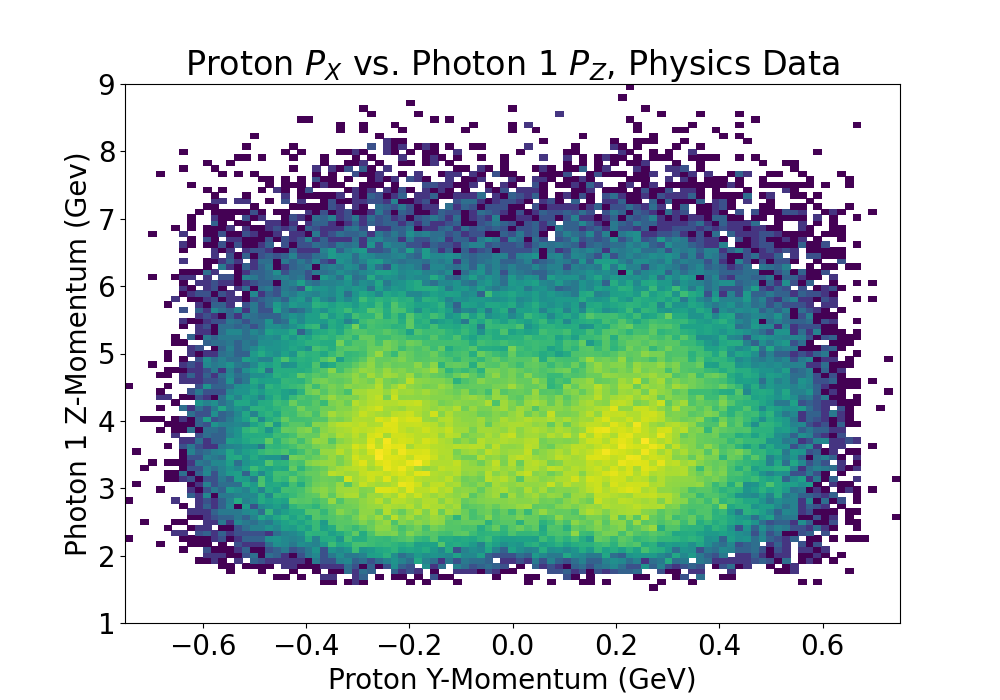
\includegraphics[width=.99\textwidth,trim={0 0 0 0},clip]{FinalPictures/Hists2D/Proton_P_X_vs_Photon_1_P_Z,_Physics_Data.png}
        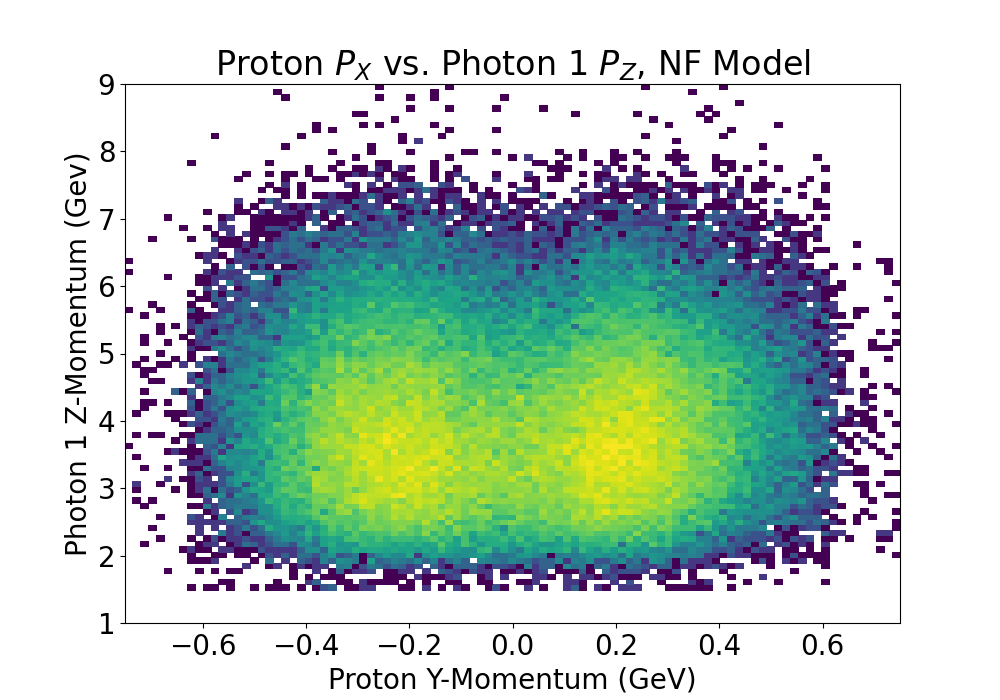
\includegraphics[width=.99\textwidth,trim={0 0 0 0},clip]{FinalPictures/Hists2D/Proton_P_X_vs_Photon_1_P_Z,_NF_Model.png}

        %\caption{(c)}
    \end{minipage}%
    \begin{minipage}{0.33\textwidth}
        \centering
       %Feature Distributions from Traditional Microphysics Simulations
        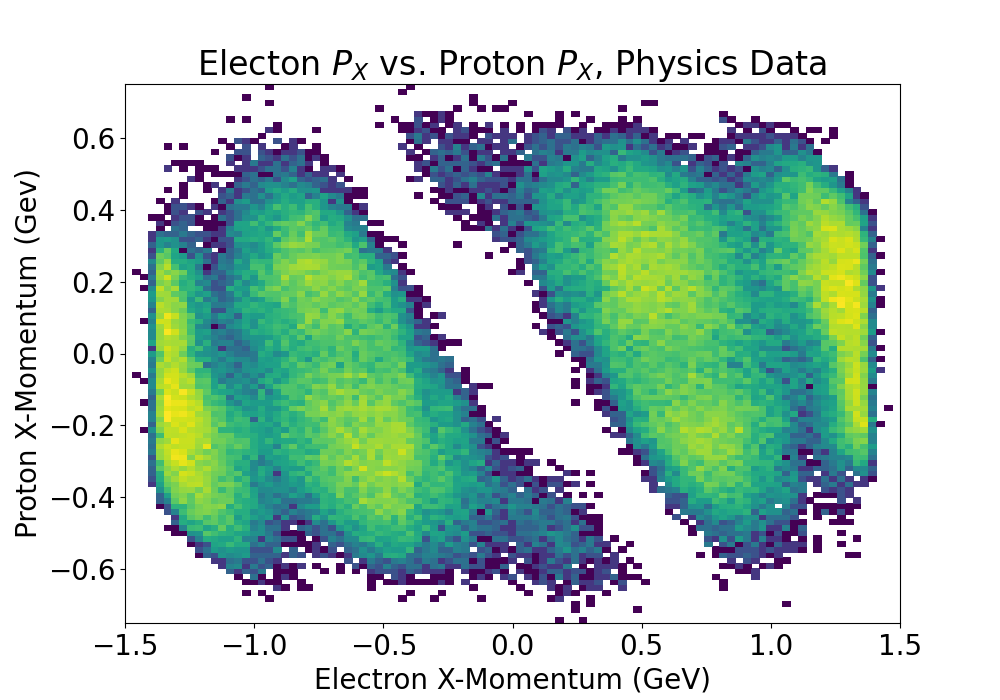
\includegraphics[width=.99\textwidth,trim={0 0 0 0},clip]{FinalPictures/Hists2D/Electon_P_X_vs_Proton_P_X,_Physics_Data.png}
        %Feature Distributions from NF Model Samples
        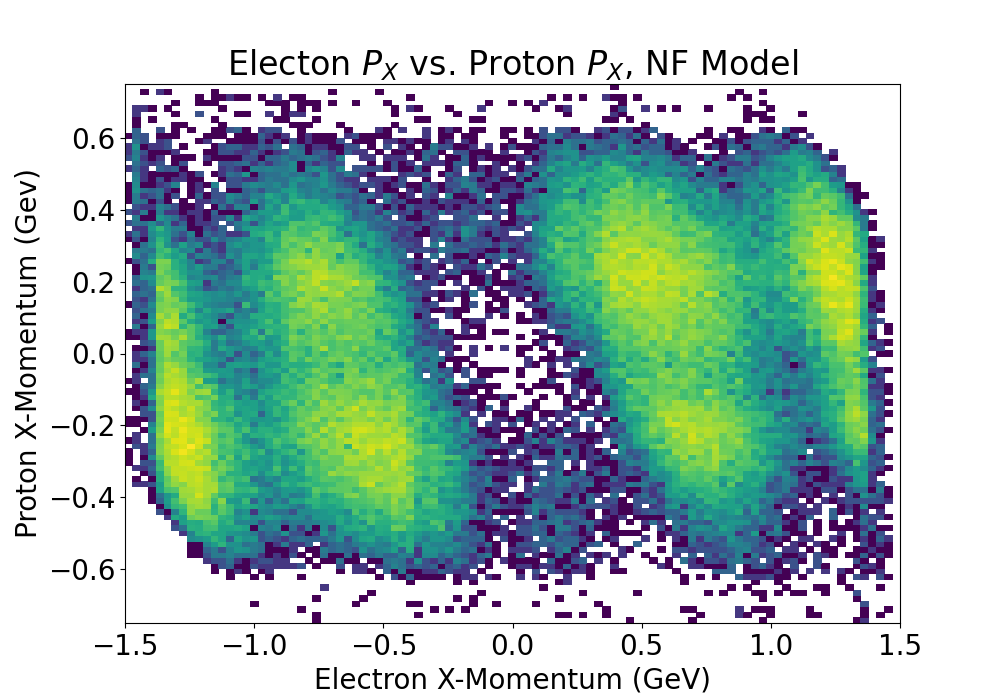
\includegraphics[width=.99\textwidth,trim={0 0 0 0},clip]{FinalPictures/Hists2D/Electon_P_X_vs_Proton_P_X,_NF_Model.png}
        %\caption{(a)}
        

    \end{minipage}
     \begin{minipage}{0.33\textwidth}
            \centering
           % Photon 1
            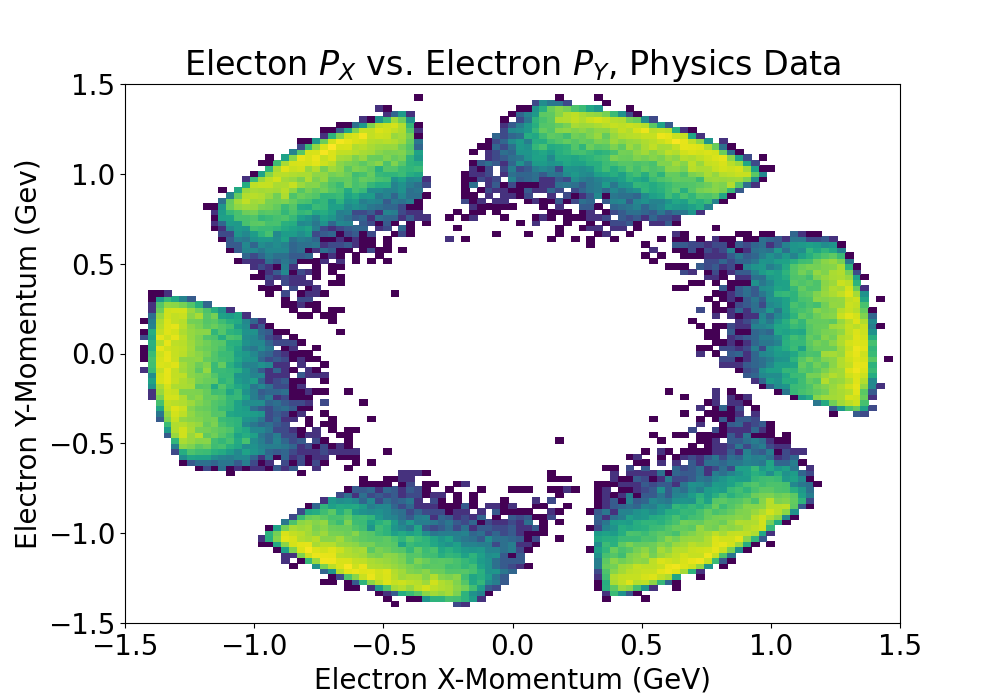
\includegraphics[width=.99\textwidth,trim={0 0 0 0},clip]{FinalPictures/Hists2D/Electon_P_X_vs_Electron_P_Y,_Physics_Data.png}
            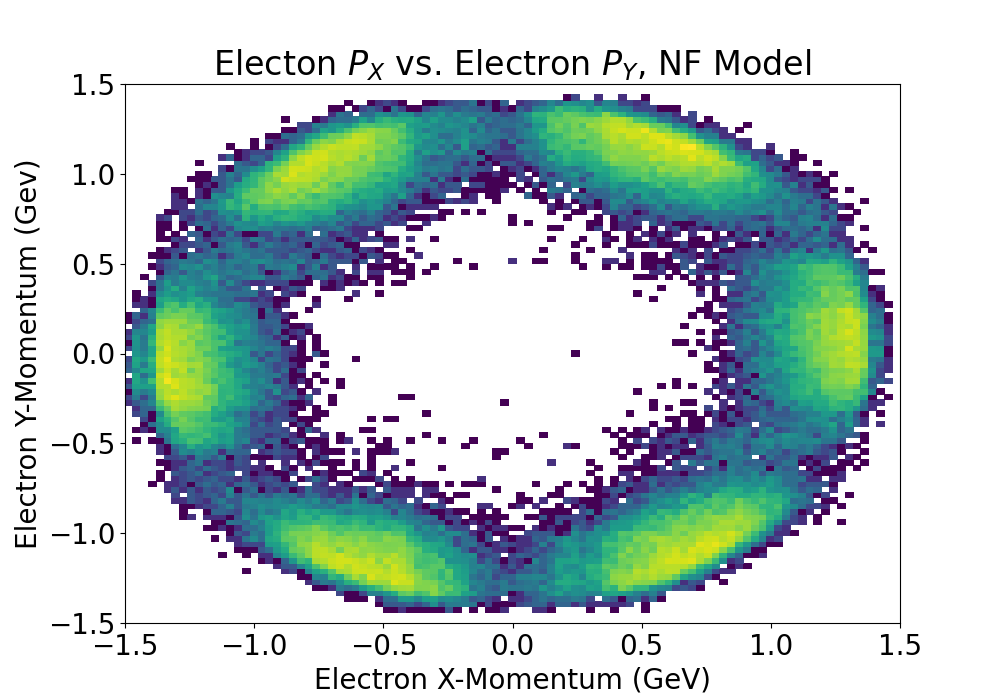
\includegraphics[width=.99\textwidth,trim={0 0 0 0},clip]{FinalPictures/Hists2D/Electon_P_X_vs_Electron_P_Y,_NF_Model.png}

    \end{minipage}
    \caption{ 2-Dimensional distributions for various features, comparing the data from the traditional physics simulation to the NF sampled data. \textbf{Top} Feature distributions from the traditional physics data set. \textbf{Bottom} Feature distributions from our trained NF model, which should match with the top row. Moving from left to right, we can see that some feature distributions are reproduced well, while others have difficult details that are not well modeled, corresponding to physical detector geometry and physics constraints that the NF model is unaware of. }
    \label{fig:2D}
\end{figure}


\subsection{Results from 4-Feature Trained NF Model}

To try to improve fine-detail reproduction by our model, we trained a second model with only 4-features, which corresponded to a full description of a simulated electron. We observed some improvement in the fidelity of feature reproduction, in particular, Figure \ref{fig:EMD2} shows that, compared to the 16-feature trained model, the 4-feature model (trained only on electron features) exhibits a 2-4 times lower EMD. Of course, this 4-feature trained model is much more limited in scope, but also is able to produce samples much faster, at a rate of about 170 Hz, compared to 4 Hz for the 16-feature model. Given that it describes fully a simulated electron, this would be useful for generally speeding up simulations, but the correlations between different particles that define specific processes like DV$\pi$P is lost. 


\begin{figure}[!h]
    \centering
    %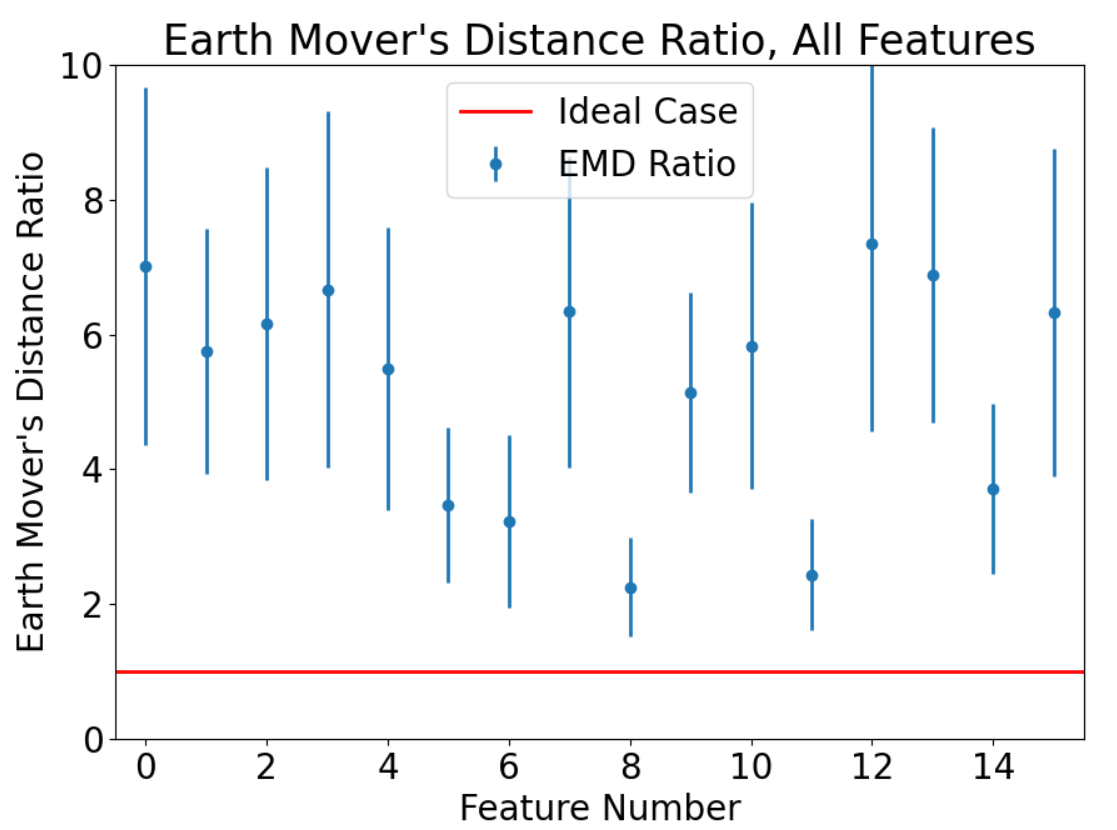
\includegraphics[scale=0.3]{FinalPictures/EMD/EmdRatio.png}
    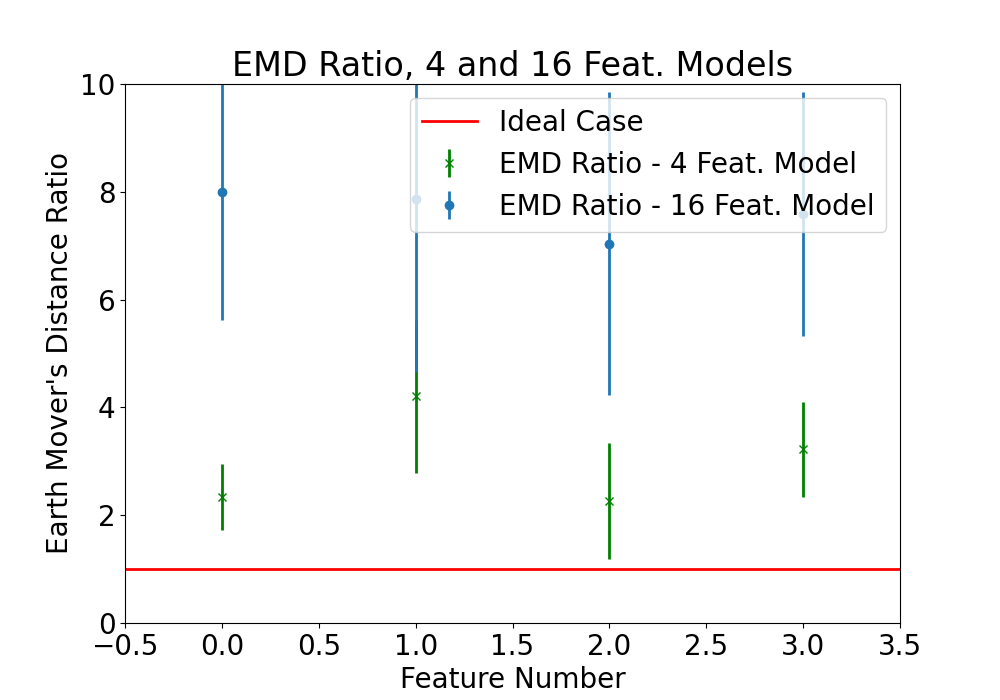
\includegraphics[width=.7\textwidth,trim={ 0 0 0 0},clip]{FinalPictures/EMD/emdratio416.png}
    \caption{The EMD Ratio of selected 4 features between the NF generated distributions and sample from physics simulation when the model was trained using all 16 features as Fig.~\ref{fig:EMD} (blue), and the selected 4 features (green). The 4-Feature trained model shows consistently lower EMD ratio values than the 16-trained model, indicating a better ability to reproduce electron features.}
    \label{fig:EMD2}
\end{figure}

Comparing to Figure \ref{fig:2D}, we can see from Figure \ref{2D4F} that the 4-feature trained NF model also demonstrates better reproduction of the sharp cutoffs in distributions caused by detector and physics constraints, although still the match is not perfect. Work is ongoing to directly include these constraints in the NF training to decrease these discrepancies.

\begin{figure}[!ht]
    \centering
     \begin{minipage}{0.323\textwidth}
        \centering
        Traditional Simulation
        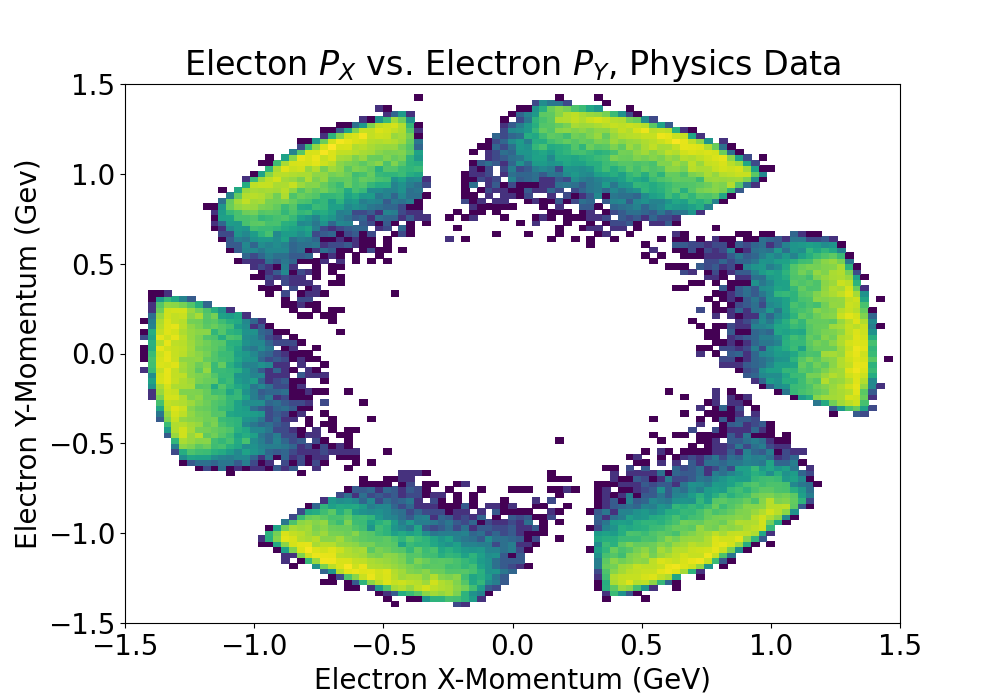
\includegraphics[width=.99\textwidth,trim={0 0 0 0},clip]{FinalPictures/Hists2D/Electon_P_X_vs_Electron_P_Y,_Physics_Data.png}
        
    \end{minipage}
         \begin{minipage}{0.323\textwidth}
        \centering
        16-Feature Model
        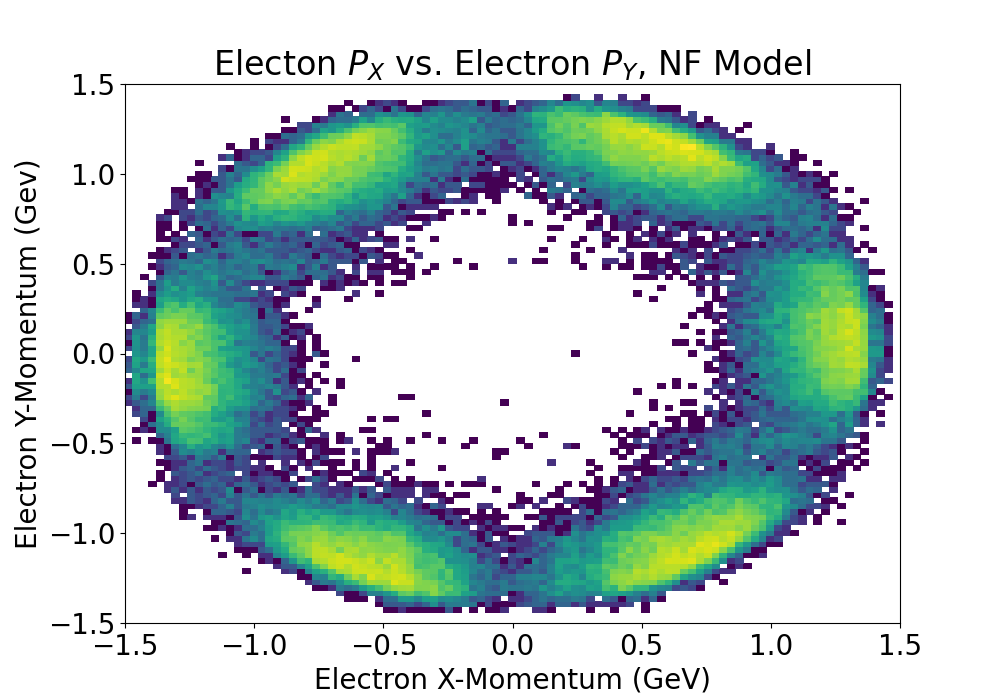
\includegraphics[width=.99\textwidth,trim={0 0 0 0},clip]{FinalPictures/Hists2D/Electon_P_X_vs_Electron_P_Y,_NF_Model.png}

    \end{minipage}
         \begin{minipage}{0.323\textwidth}
        \centering
        4-Feature Model
       
        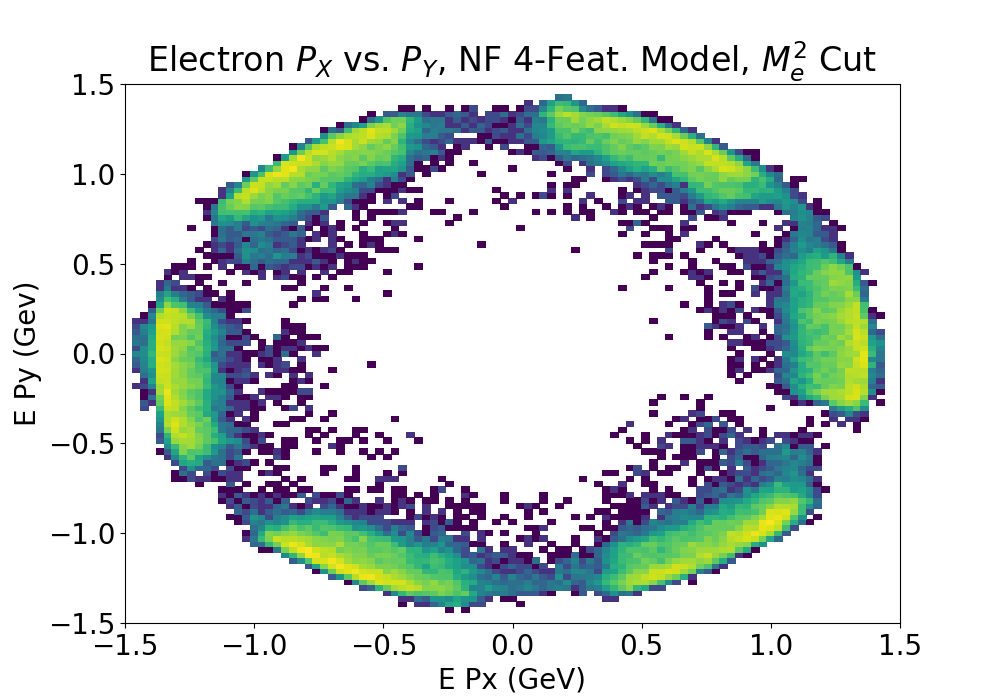
\includegraphics[width=.99\textwidth,trim={0 0 0 0},clip]{FinalPictures/2D_Hists_4F/Electron_P_X_vs_P_Y,_NF_4-Feat_Model,_M_e2_Cut.png}
    \end{minipage}
    \caption{\textbf{Left}: Electron X-Momentum vs. Electron Y-Momentum distribution from the traditional physics simulation dataset. \textbf{Center}: The observed distribution from the 16-Feature trained model, copied from Figure \ref{fig:2D} for reference. We can see considerable disparity between this distribution and the traditional physics distribution. \textbf{Right}: The distribution result from the 4-Feature trained model, which demonstrates far greater agreement to the traditional results compared to the 16-Feature model. }
    \label{fig:2D4F}
\end{figure}

\clearpage

\subsection{Utilizing NF Model Samples for Physics Analysis}

Ultimately, we are interested in physics processes rather than just distribution mapping, so we also examined our ability to reconstruct physics quantities from the trained NF model sample data. Figure \ref{fig:protonspions} shows the distribution of calculated proton and pion (calculated from a combination of the photon features) masses from our NF model data, which had no explicit physics constraints in training. We observe a peak at about 0.939 GeV for the proton and 0.136 GeV for the pion, , which is within 0.5\% of the value encapsulated in the traditional physics training dataset. 


\begin{figure}[!h]
    \centering
    %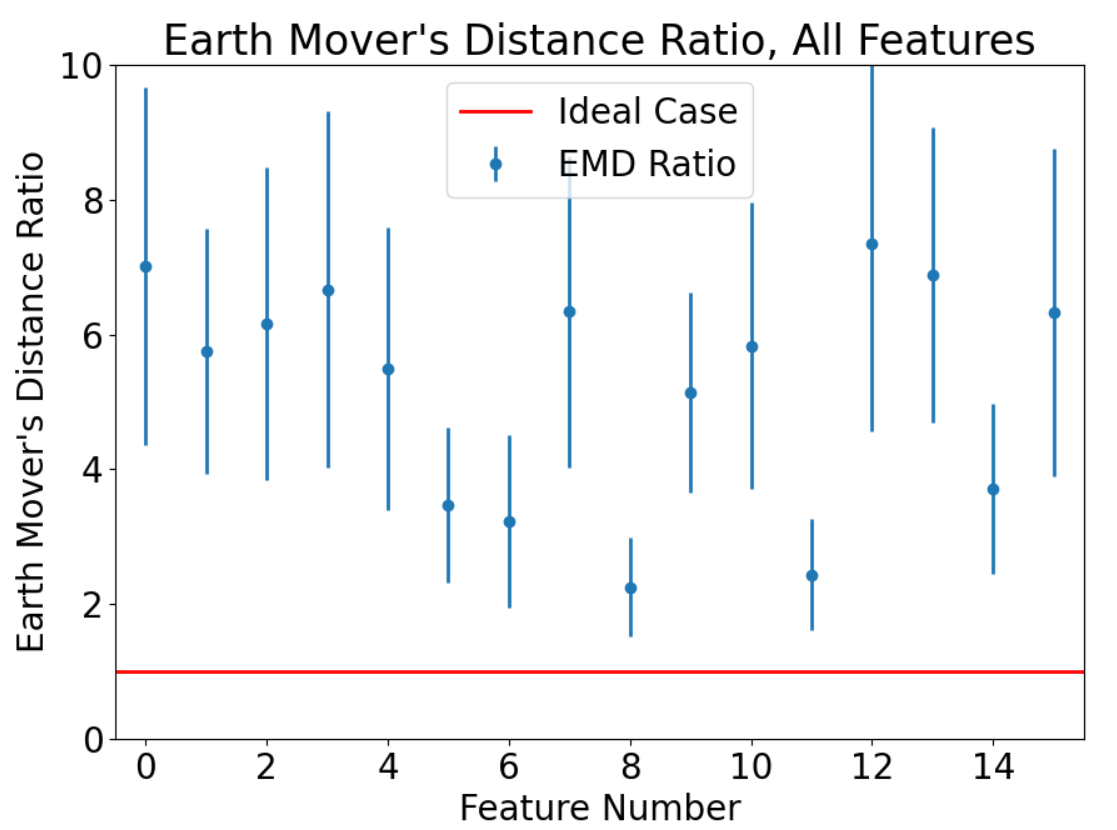
\includegraphics[scale=0.3]{FinalPictures/EMD/EmdRatio.png}
    

    \label{fig:protons}
\end{figure}



\begin{figure}[!ht]
    \centering
     \begin{minipage}{0.49\textwidth}
        \centering
        %Photon 2
        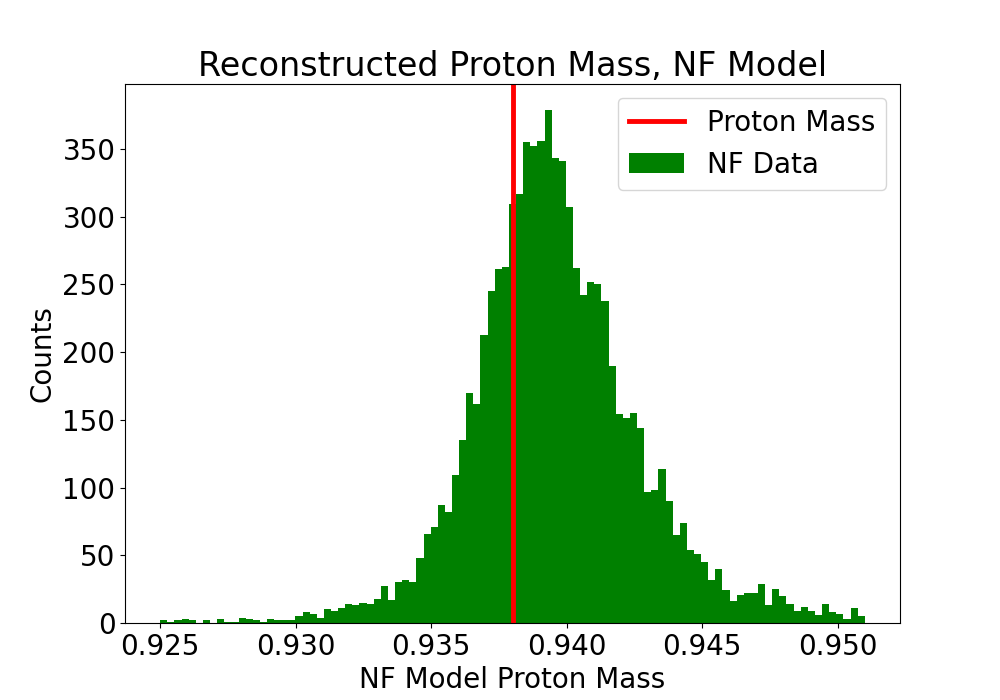
\includegraphics[width=.97\textwidth,trim={ 0 0 0 0},clip]{FinalPictures/protons}

    \end{minipage}
    \begin{minipage}{0.45\textwidth}
        \centering
        %Photon 2
        
        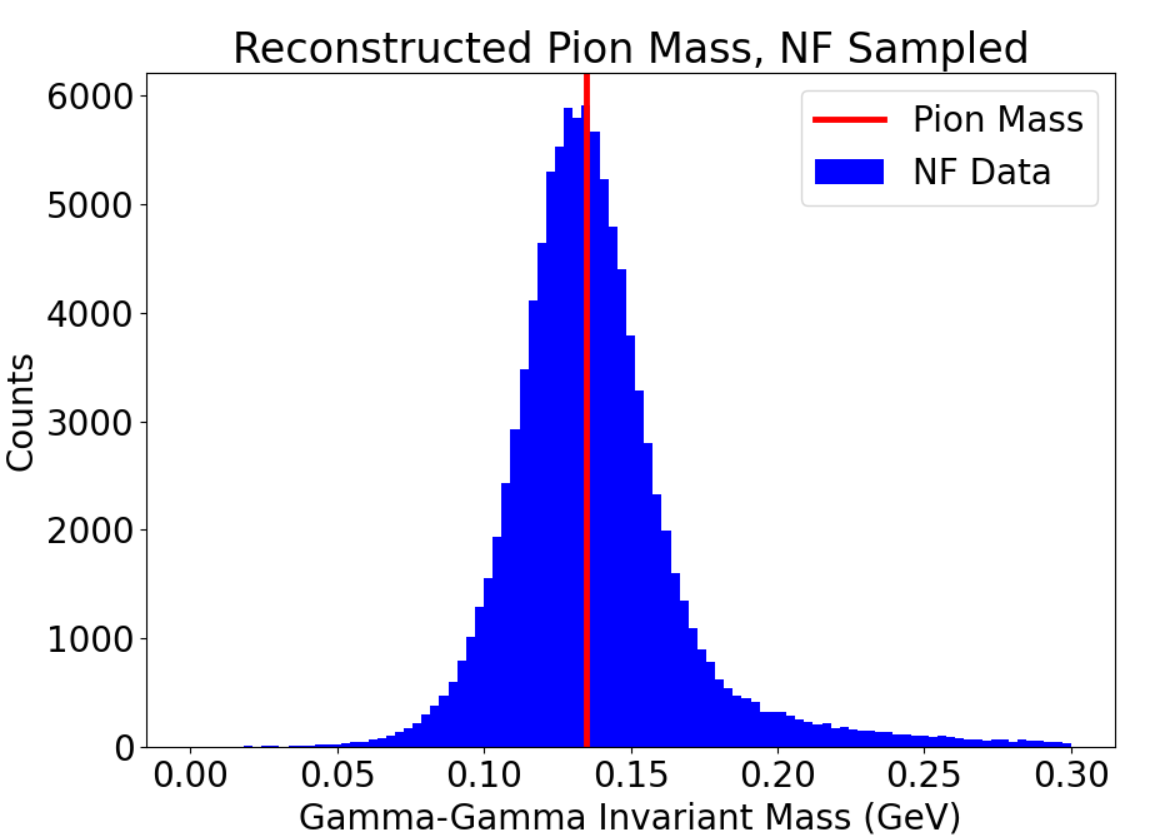
\includegraphics[width=.97\textwidth,trim={ 0 0 0 0},clip]{FinalPictures/pions}
    \end{minipage}
        \caption{The distributions of calculated proton mass (left) and pion mass (right) from the 16-Feature trained NF model.  The accepted (true) particle masses are indicated by the red vertical lines, at 0.938 GeV and 0.135 GeV, respectively. The peaks from the model are about 1 MeV, or about 0.5\%, shifted away from these true values; while this is small, it is currently unclear what is causing this shift.}
    \label{fig:protonspions}
\end{figure}


\section{Conclusion}

Overall, we are able to use a UMNN-MAF architecture to attain reasonable physics distributions far faster than just using traditional physics simulations. At this stage, it is not clear if the 10x speedup afforded by the 16-feature NF model is sufficiently large to justify a decrease in fine-detail resolution. Work is ongoing as to if the model resolution can be improved by including conservation laws as part of training, or if the model can be optimized to generate samples faster. 

On the other hand, the 4-feature model has both higher resolution, and is able to produce samples 1,000 times faster than traditional methods, and so could be very useful immediately to physics research efforts. However, as it is only 4-features, it can only represent one particle, not an entire physics process, but this is still relevant to the study of background processes and noise events in physics experiments, and we are investigating applying this to current CLAS12 research.

The ability of the 16-Feature model to produce realistic protons and pions demonstrates viability for using this method in real physics analysis, but we show there are fine details that the model cannot learn without additional constraints. Work is ongoing to incorporate the physical experimental layout and physics conservation laws into the flow training, which we expect will resolve these discrepancies in fine-detail reproduction, and will lead to a more accurate reproduction of the traditional simulation results, at a far faster speed. 




%\section{Discussion and Summary}

%We presented a NF model to sample data points of 4 or 16 features to replace the standard physics simulation. We expect the model to be useful for collaborators who want new random data sample of DV$\pi^0$P simulation.
%As we have observed in the previous section, \citet{NEURIPS2019_2a084e55} and \citet{papamakarios2018masked} point out that we can train the MAF model fast using 16 features in 5M rows. This is because the Masked Autoencoder for Distribution Estimation (MADE, \citet{pmlr-v37-germain15}), which is a building block of MAF allows the training to be done in parallel using GPUs. In the mean time, sampling data points from the trained MAF takes significant amount of time because the model requires $\mathbf{z}_{i,0:j-1}$ to sample $\mathbf{z}_{i,j}$. There is a computational trade-off in Inverse Autoregressive Flow (IAF, \citet{NIPS2016_ddeebdee}, which trains the model slowly but samples fast. Despite this known drawback, we still consider the UMNN-MAF to be the optimal model for this project because training the model to sample data points following distributions reasonably close to that of physics simulation. %Unfortunately, at this stage, we do not have the reference of EMD ratio to define the good sampling.

\iffalse
\section{Preliminary Results}
Fig.~\ref{fig:a} visualizes the four features of the test data $\mathbf{x_1}$ and $\mathbf{x_2}$. For compactness we only show 2 of the 6 possible combinations of 4 features, specifically, the top row of  Fig.~\ref{fig:a} plots the distributions of features 0 and 1 (EP - electron and proton momentum) while the bottom row plots the distributions of features 2 and 3 (GG - the two photons' momentum). The 1D distributions of each feature is shown in the top row of Fig.~\ref{fig:b}'s. Qualitatively, the MAF generated data generally follows the microphysics generated data, but differ in detailed shape in some places of the distribution. At this stage it is not clear what is causing this discrepancy, or how it can be mitigated. It is possible that including more features in training will provide higher fidelity results due to the correlations between features, but this is an active area of our research. We are also investigating modifying our base distribution, and altering our hyerparameters, to resolve these details to a higher degree.

\begin{figure}[!ht]
    \centering
    \begin{minipage}{.4\textwidth}
    Feature Distribution: Physics Data
        \centering
        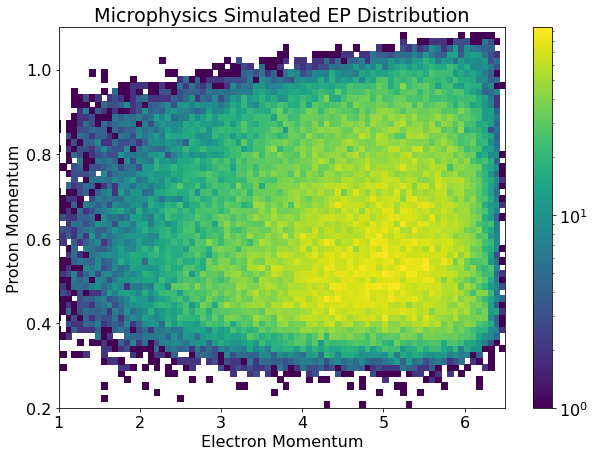
\includegraphics[width=.9\textwidth,trim={0 0 0 0},clip]{pictures/milestoneR2/gemc1.png}
        %\caption{(a)}
        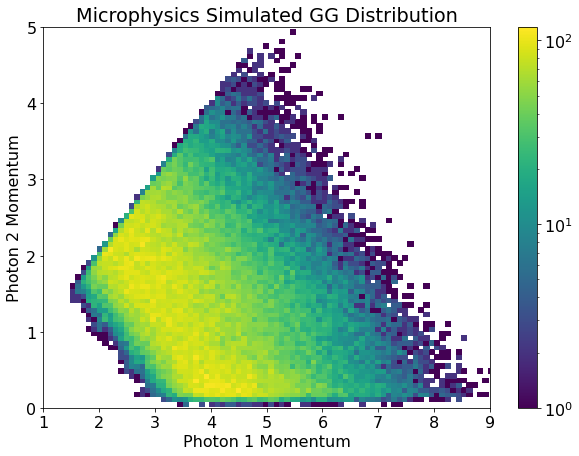
\includegraphics[width=.9\textwidth,trim={0 0 0 0},clip]{pictures/milestoneR2/gemc2.png}
        %\caption{(c)}
    \end{minipage}%
    \begin{minipage}{0.4\textwidth}
    Feature Distribution: NFlow Generated
        \centering
        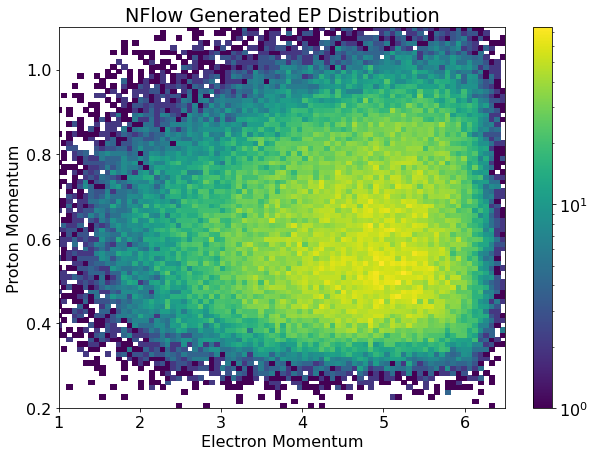
\includegraphics[width=.9\textwidth,trim={0 0 0 0},clip]{pictures/milestoneR2/nflow1.png}
        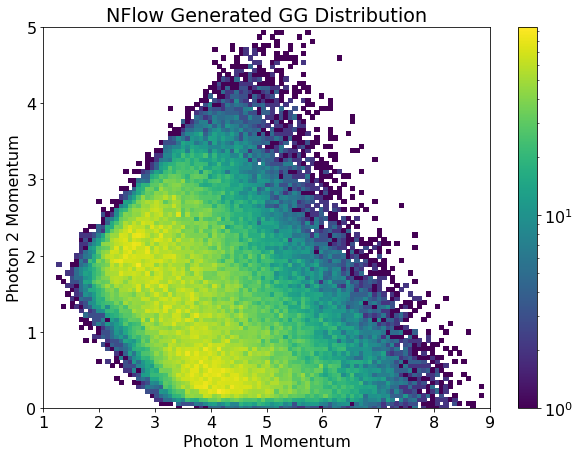
\includegraphics[width=.9\textwidth,trim={0 0 0 0},clip]{pictures/milestoneR2/nflow2.png}
    \end{minipage}
    \caption{\textbf{Left}: 2D distributions of the physics data $\mathbf{x_1}$. \textbf{Right}: 2D distributions of the data generated from the MAF $\mathbf{x_2}$.}
    \label{fig:a}
\end{figure}

\begin{figure}[!ht]
    \centering
    \begin{minipage}{1\textwidth}
    Feature Distribution: Physics Data
        \centering
        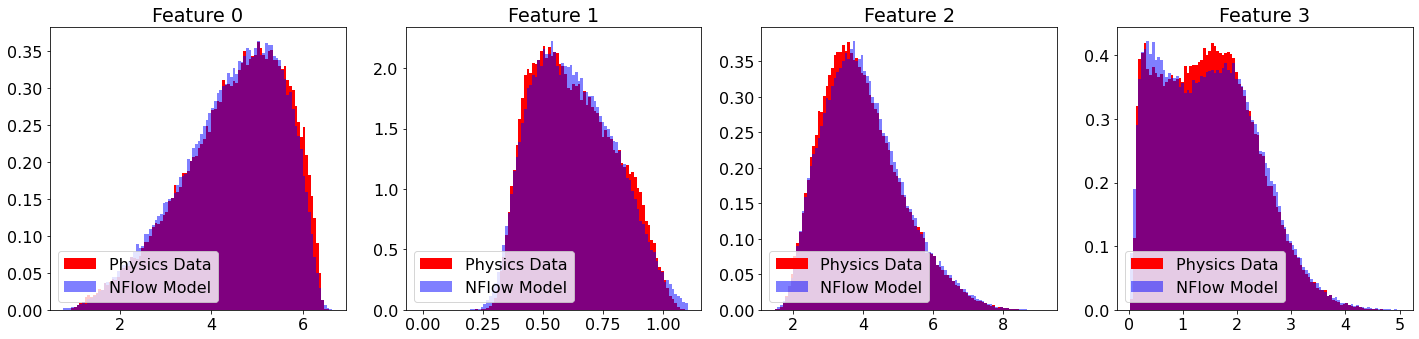
\includegraphics[width=.9\textwidth,trim={0 0 0 0},clip]{pictures/milestoneR2/comp1.png}
        %\caption{(a)}
        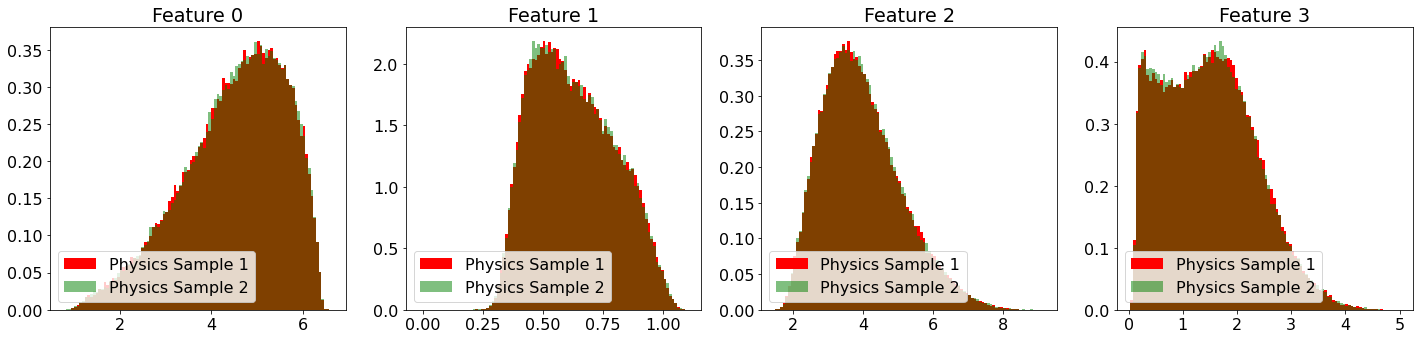
\includegraphics[width=.9\textwidth,trim={0 0 0 0},clip]{pictures/milestoneR2/comp2.png}
        %\caption{(c)}
    \end{minipage}%
    \caption{\textbf{Top}: Distributions of each feature in $\mathbf{x_1}$ (labeled as `Physics Data') and $\mathbf{x_2}$ (labeled as `NFlow Model'). \textbf{Bottom}: Comparison of distributions of each feature in $\mathbf{x_1}$ (labeled as `Physics Sample 1') and $\mathbf{x_1'}$ (labeled as `Physics Sample 2'). See Table 1 for EMD and KLD values.}
    \label{fig:b}
\end{figure}


\begin{center}
\begin{table}[ht]
\caption{EMD and KLD Values from Fig. ~\ref{fig:b}}
\centering
\begin{tabular}{ |p{2.5cm}||p{1.4cm}|p{1.4cm}|p{1.4cm} |p{1.4cm}| }

 %\hline
 %\multicolumn{5}{|c|}{Values of EMD and KLD for Fig.~\ref{fig:b}} \\ 
 \hline
%Quantity &  \multicolumn{4}{|c|}{Feature Number} \\ 
\textbf{Quantity} & \textbf{Feature 0} & \textbf{Feature 1} & \textbf{Feature 2} & \textbf{Feature 3} \\
 \hline                                             
%\multirow{2}{4em}{EMD}  & 0.0671 & 0.0048 & 0.0469 & 0.03533\\ 
EMD - NFlow  & 0.0671 & 0.0048 & 0.0469 & 0.0353\\ 
EMD - Sample & 0.0111 & 0.0006 & 0.0148 & 0.0038\\ 

\hhline{|=|=|=|=|=|}
%\multirow{2}{4em}{KLD} & $\infty$ & 0.0748 & 0.07969 & $\infty$\\ 
KLD- NFlow & $\infty$ & 0.0748 & 0.07969 & $\infty$\\ 
KLD - Sample & 0.0721 & 0.0730 & 0.07962 & 0.3973 \\ 

 \hline
\end{tabular}
\end{table}
\end{center}

\iffalse
\begin{center}
\begin{tabular}{c c c c c c }
Quantity & F0 & F1 & F2 & F3  \\
\hline
NFlow EMD & 0.0671 & 0.0048 & 0.0469 & 0.0353 \\ 
Sample EMD & 0.0111 & 0.0006 & 0.0148 & 0.0038 \\
NFlow KLD & $\infty$ & 0.0748 & 0.07969 & $\infty$\\  
Sample KLD & 0.0721 & 0.0730 & 0.07962 & 0.3973\\ 
\end{tabular}
\end{center}
\fi

Examining Table 1, we can see that our model is performing reasonably, with room to improve. Note that we did not restrict the flow to generate data only in regions of phase space where data exists for the physics set, so it is possible to have infinite divergence for the KLD value, although it is not helpful. Where it is well defined, we see very similar values between the MAF generated dataset $\mathbf{x_2}$ and the comparison dataset $\mathbf{x_1'}$. The EMD is defined at all times in our process, and so it is very useful, and indicates a somewhat worse agreement between our model and a perfect replica of the distribution. 


\begin{figure}[!ht]
    \centering
    \begin{minipage}{.25\textwidth}
    
        \centering
        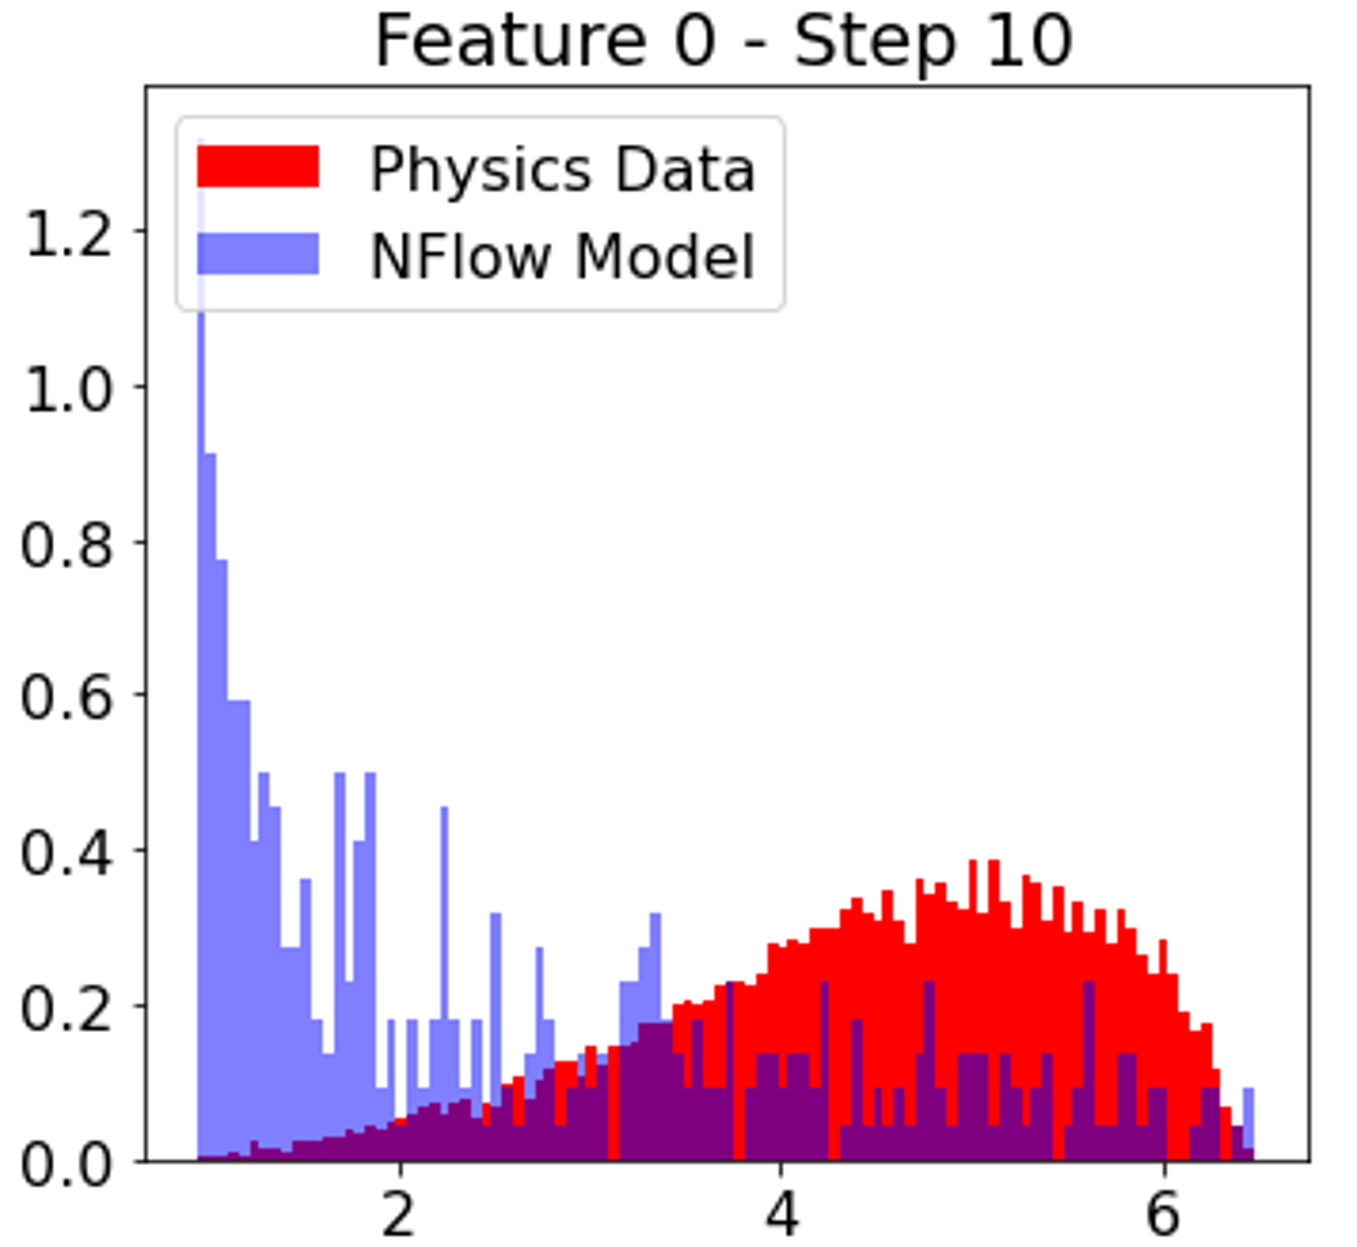
\includegraphics[width=.9\textwidth,trim={0 0 0 0},clip]{pictures/milestoneR2/steps/s10.png}
        %\caption{(a)}
        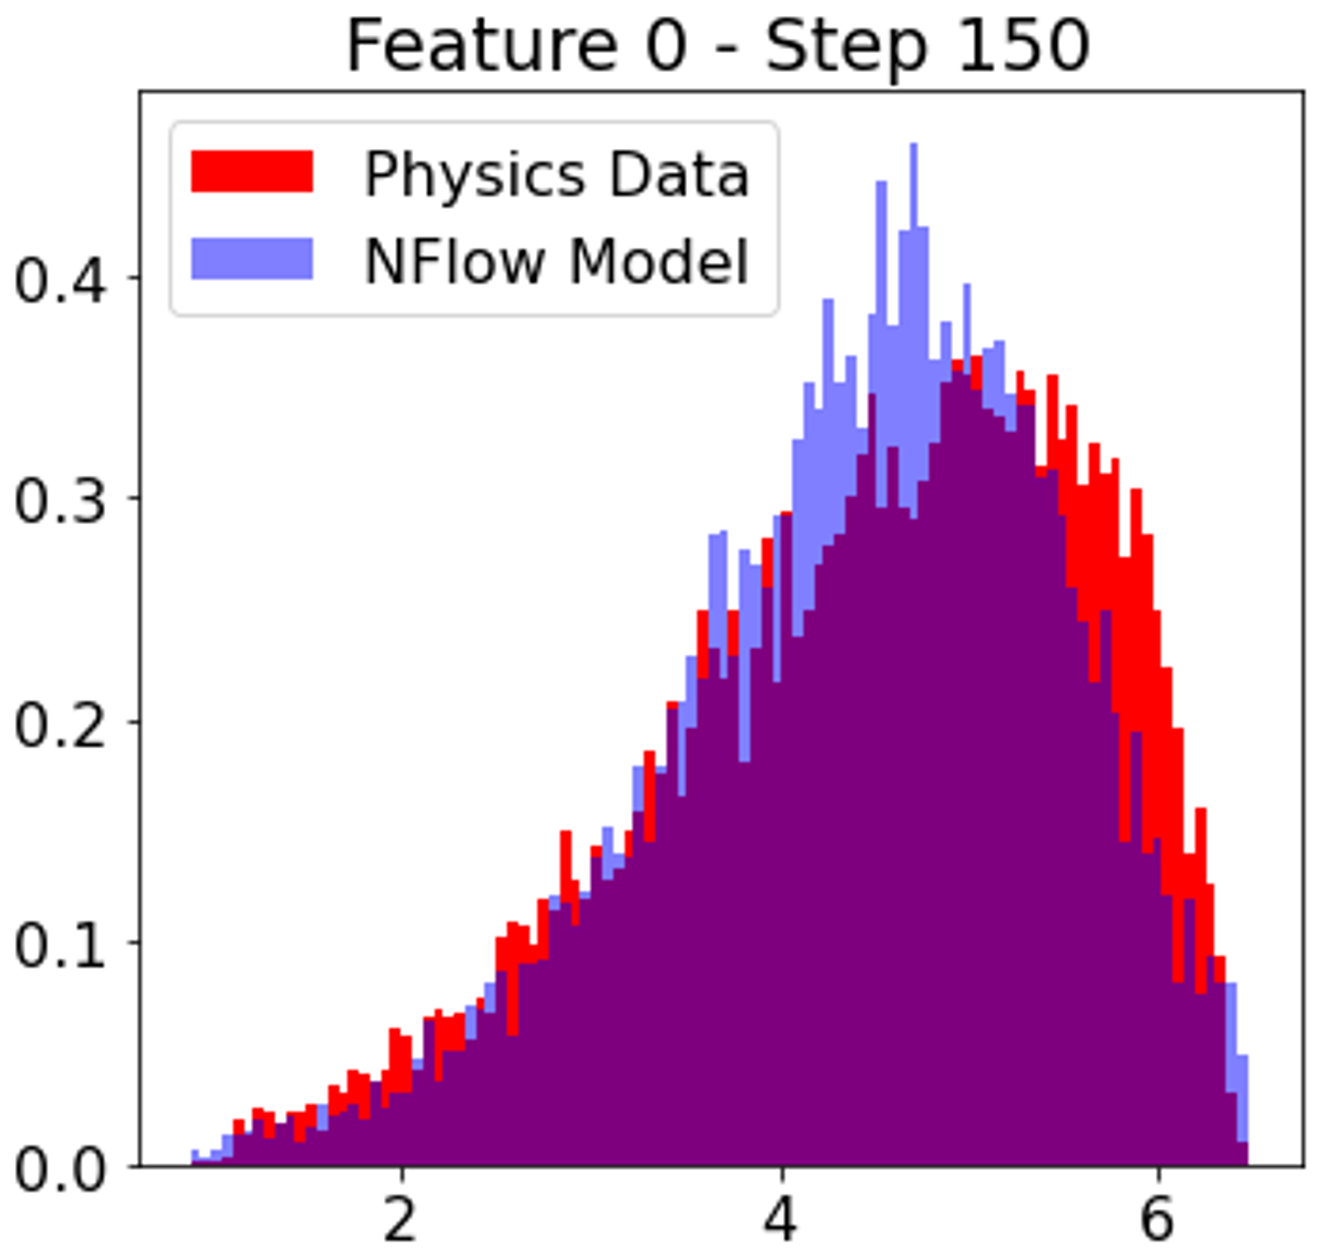
\includegraphics[width=.9\textwidth,trim={0 0 0 0},clip]{pictures/milestoneR2/steps/s150.png}
        %\caption{(c)}
    \end{minipage}%
    \begin{minipage}{0.25\textwidth}
    
        \centering
        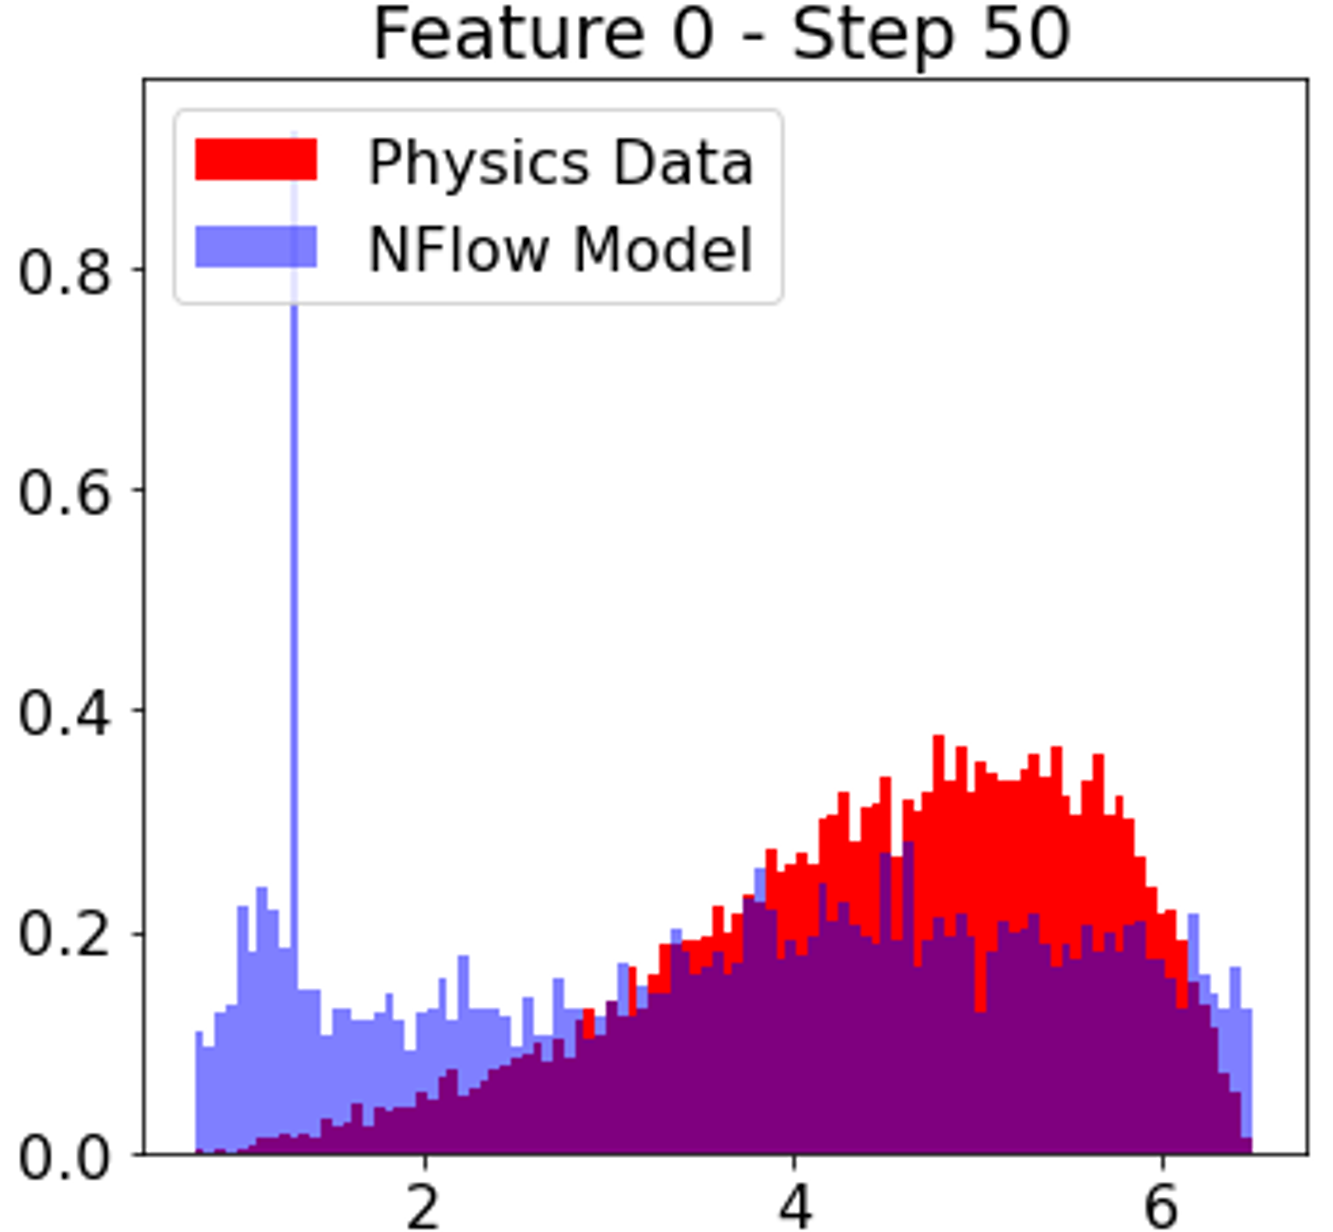
\includegraphics[width=.9\textwidth,trim={0 0 0 0},clip]{pictures/milestoneR2/steps/s50.png}
        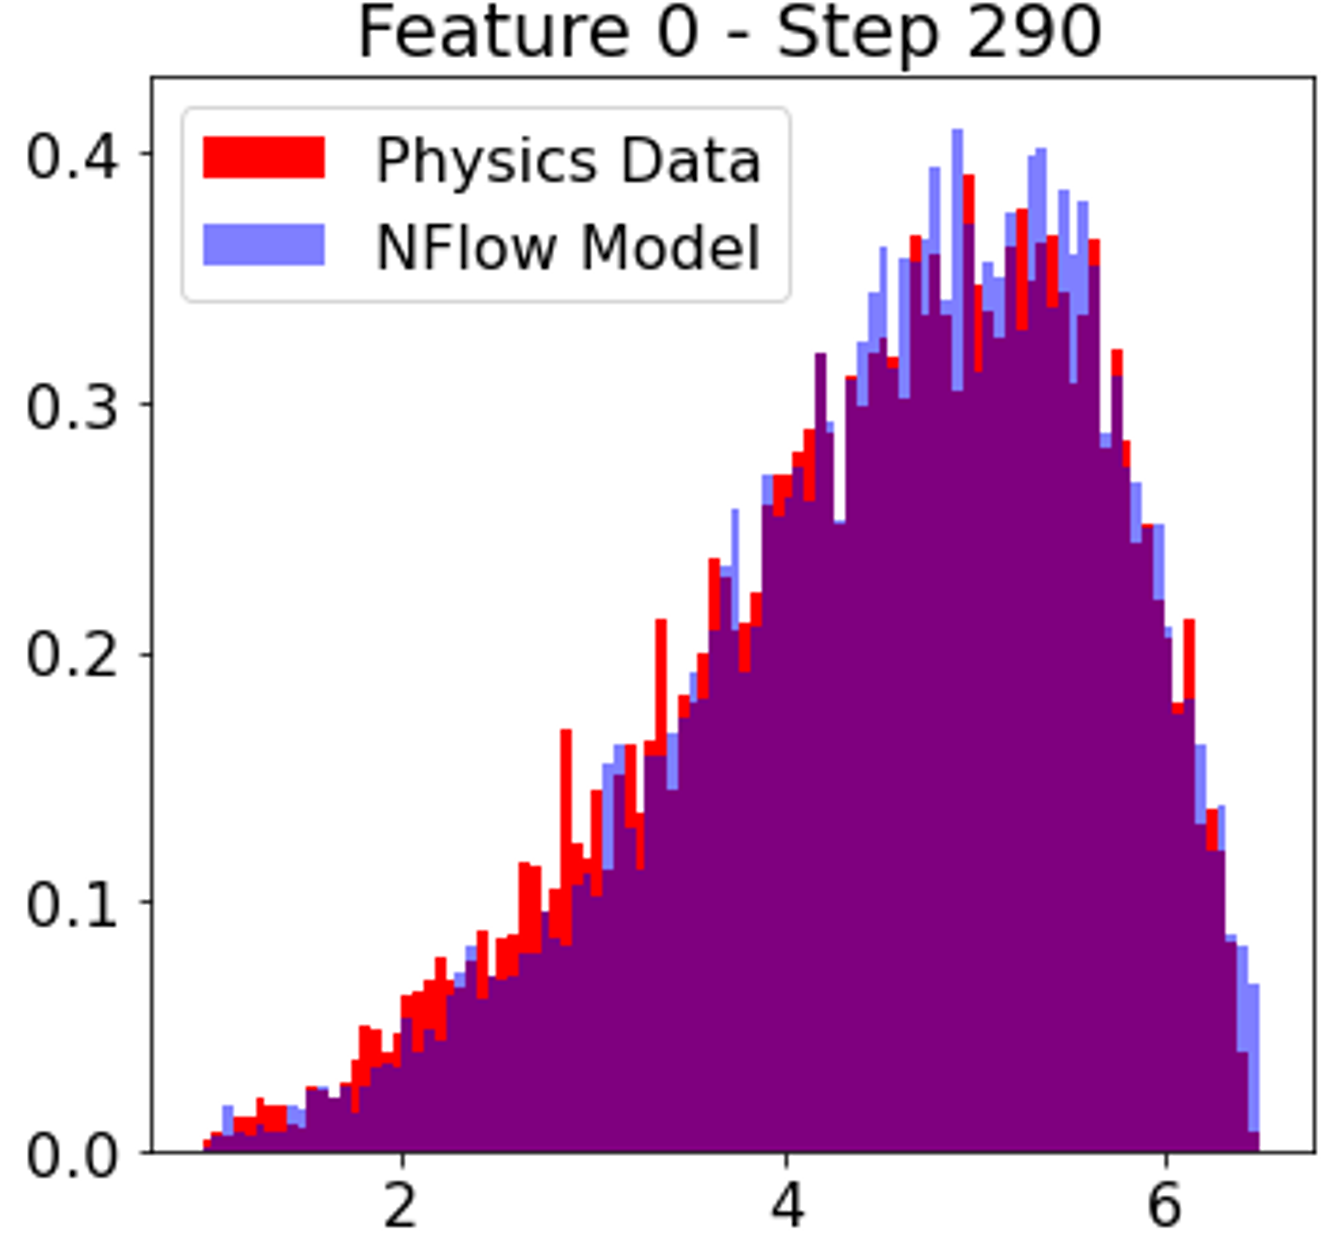
\includegraphics[width=.9\textwidth,trim={0 0 0 0},clip]{pictures/milestoneR2/steps/s290.png}
    \end{minipage}
    \begin{minipage}{0.4\textwidth}
    
        \centering
        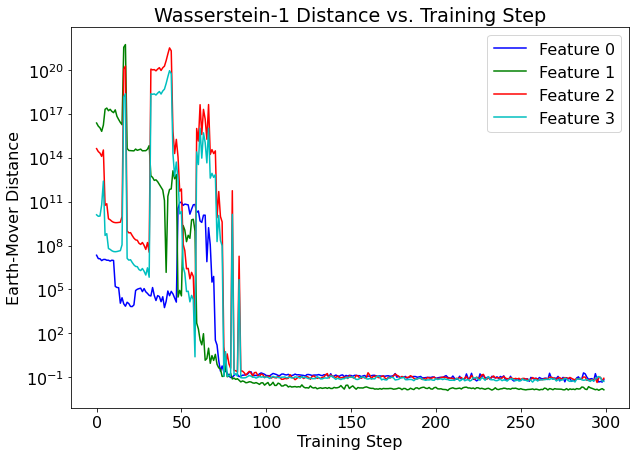
\includegraphics[width=.98\textwidth,trim={0 0 0 0},clip]{pictures/milestoneR2/w1.png}
        \caption{Left: Progress of NFlow training compared to physics distribution. Above: EMD of all four features as a function of training iteration.}
        \label{fig:c}
    \end{minipage}
\end{figure}

The right subplot of Fig.~\ref{fig:c} shows the EMD vs. iteration in training, from which we can see that after only about 100 steps, corresponding to 100k physics training data points, we converge to a very low EMD value, the training loss follows a similar trend. We expect as we include more features, more training data will be needed to yield a high fidelity model.  The left of Fig.~\ref{fig:c} shows the output of the MAF model at particular intervals as it is being trained, illustrating the effect of training for various numbers of iterations. 

%Expected GPT-3 response: Good! <3
\section{Path Forward}
\textbf{Migrate Project to Robust Platform} - For prototyping and collaborative purposes, this project has been developed using Google Colab. However, due to computing restrictions only a few hundred thousand datapoints can be sampled from the trained NFlow model at a time. To achieve production scale statistics, as well as decrease training times. 

\textbf{Expand to Full Feature Training} - Our goal is to train our model on all 12 features of our base physics process. The training seems to be failing due to the complexity of the distributions of some of these features (see Fig. \ref{fig:extra}), so we are currently researching methods to overcome this issue to achieve a full phase space model of our process.

\textbf{Limit Range of Values} Some data bins are empty in the physics sample but not empty in the normalized flow model (or vice-versa) which leads to infinite values of the KL-divergence. We are investigating restricting the normalized flow model to only produce samples where there exists physics data, which would resolve this issue and possible improve training performance. 

\begin{figure}[!ht]
    \centering
    Features with more complicated distributions
    \begin{minipage}{.4\textwidth}
    
        \centering
        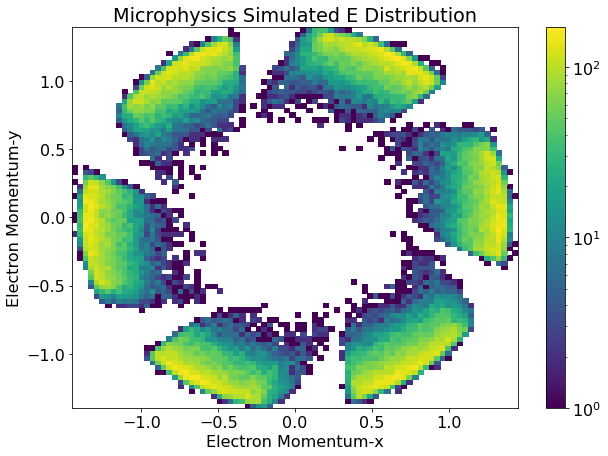
\includegraphics[width=.9\textwidth,trim={0 0 0 .875cm},clip]{pictures/milestoneR2/pxpy/epxpy.png}
        %\caption{(a)}
        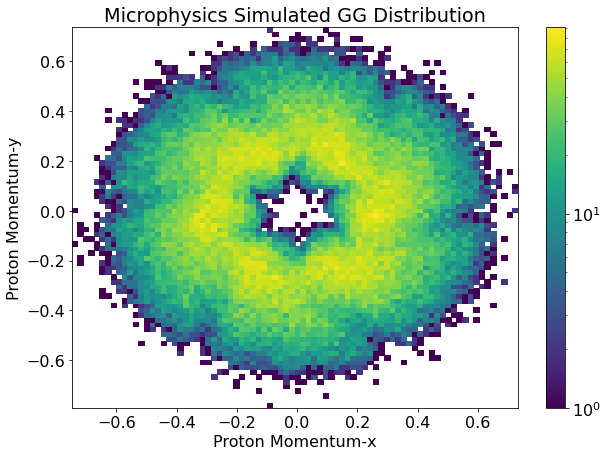
\includegraphics[width=.9\textwidth,trim={0 0 0 .875cm},clip]{pictures/milestoneR2/pxpy/ppxpy.png}
        %\caption{(c)}
    \end{minipage}%
    \begin{minipage}{0.4\textwidth}
    
        \centering
        \includegraphics[width=.9\textwidth,trim={0 0 0 .875cm},clip]{pictures/milestoneR2/pxpy/g2pxpy.png}
        \includegraphics[width=.9\textwidth,trim={0 0 0 .875cm},clip]{pictures/milestoneR2/pxpy/gpxpy.png}
    \end{minipage}
    \caption{Nontrivial feature distributions from physics data that are yet to be modeled successfully by the NFlow model.}
    \label{fig:extra}
\end{figure}


\iffalse
Path forward:\\
Utilization of "z" distribution to train prior distribution\\
Expand to full feature representation learning\\
\fi


\iffalse
Parameters for best run:

prior = TransformedDistribution(Uniform(torch.zeros(2), torch.ones(2)), SigmoidTransform().inv) # Logistic distribution
#prior = MultivariateNormal(torch.zeros(2), torch.eye(2))
# NICE
flows = [AffineHalfFlow(dim=2, parity=i%2, scale=False) for i in range(12)] 
33

#print(flows)
flows.append(AffineConstantFlow(dim=2, shift=False))
#print(flows)


# construct the model
model = NormalizingFlowModel(prior, flows)

optimizer = optim.Adam(model.parameters(), lr=5e-4, weight\_decay=1e-9)
for k in range(5000):
    sampleDict = xz.sample(1000)
    

 Path forward:
 working just on google colab, we quickly run into computing performance issues
 \fi
 
 \fi
 


\clearpage
\small
\bibliographystyle{unsrtnat}
\bibliography{references}
% [1] Alexander, J.A.\ \& Mozer, M.C.\ (1995) Template-based algorithms for
% connectionist rule extraction. In G.\ Tesauro, D.S.\ Touretzky and T.K.\ Leen
% (eds.), {\it Advances in Neural Information Processing Systems 7},
% pp.\ 609--616. Cambridge, MA: MIT Press.

% [2] Bower, J.M.\ \& Beeman, D.\ (1995) {\it The Book of GENESIS: Exploring
%   Realistic Neural Models with the GEneral NEural SImulation System.}  New York:
% TELOS/Springer--Verlag.

% [3] Hasselmo, M.E., Schnell, E.\ \& Barkai, E.\ (1995) Dynamics of learning and
% recall at excitatory recurrent synapses and cholinergic modulation in rat
% hippocampal region CA3. {\it Journal of Neuroscience} {\bf 15}(7):5249-5262.

\end{document}